\documentclass[a4paper, 12pt]{article}

%%% SST LAB PROTOCOLL PREAMBLE
%%% 2019
%%%%%%%%%%%%%%%%%%%%%%%%%%%%%%%


%%% PACKAGES
%%%%%%%%%%%%%%%%%%%%%%%%%%%

\usepackage[ngerman]{babel}

\usepackage[utf8]{inputenc}
\usepackage{amsmath}
\usepackage{pgfplots}
\usepackage{tikz}
\usepackage[many]{tcolorbox}
\usepackage{graphicx}
\graphicspath{ {./graphics/} }
\usepackage{pdfpages}
\usepackage{dashrule}
\usepackage{float}
\usepackage{siunitx}
\usepackage{trfsigns}
\usepackage{booktabs}
\usepackage[european]{circuitikz}
\usepackage{tcolorbox}

%%% DOCUMENT GEOMETRY
%%%%%%%%%%%%%%%%%%%%%%%%%%%

\usepackage{geometry}
\geometry{
 a4paper,
 total={0.6180339887498948\paperwidth,0.6180339887498948\paperheight},
 top = 0.1458980337503154\paperheight,
 bottom = 0.1458980337503154\paperheight
 }
\setlength{\jot}{0.013155617496424828\paperheight}
\linespread{1.1458980337503154}

\setlength{\parskip}{0.013155617496424828\paperheight} % paragraph spacing


%%% COLORS
%%%%%%%%%%%%%%%%%%%%%%%%%%%

\definecolor{red1}{HTML}{f38181}
\definecolor{yellow1}{HTML}{fce38a}
\definecolor{green1}{HTML}{95e1d3}
\definecolor{blue1}{HTML}{66bfbf}
\definecolor{hsblue}{HTML}{00b1db}
\definecolor{hsgrey}{HTML}{afafaf}

%%% CONSTANTS
%%%%%%%%%%%%%%%%%%%%%%%%%%%
\newlength{\smallvert}
\setlength{\smallvert}{0.0131556\paperheight}


%%% COMMANDS
%%%%%%%%%%%%%%%%%%%%%%%%%%%

% differential d
\newcommand*\dif{\mathop{}\!\mathrm{d}}

% horizontal line
\newcommand{\holine}[1]{
  	\begin{center}
	  	\noindent{\color{hsgrey}\hdashrule[0ex]{#1}{1pt}{3mm}}\\%[0.0131556\paperheight]
  	\end{center}
}

% mini section
\newcommand{\minisec}[1]{ \noindent\underline{\textit {#1} } \\}

% quick function plot
\newcommand{\plotfun}[3]{
  \vspace{0.021286\paperheight}
  \begin{center}
    \begin{tikzpicture}
      \begin{axis}[
        axis x line=center,
        axis y line=center,
        ]
        \addplot[draw=red1][domain=#2:#3]{#1};
      \end{axis}
    \end{tikzpicture}
  \end{center}
}

% box for notes
\newcommand{\notebox}[1]{

\tcbset{colback=white,colframe=green1!100!black,title=Note!,width=0.618\paperwidth,arc=0pt}

 \begin{center}
  \begin{tcolorbox}[]
   #1 
  \end{tcolorbox}
 
 \end{center} 
 
}

% box for equation
\newcommand{\eqbox}[2]{
	
	\tcbset{colback=white,colframe=green1!100!black,title=,width=#2,arc=0pt}
	
	\begin{center}
		\begin{tcolorbox}[ams align*]
				#1
		\end{tcolorbox}
		
	\end{center} 
	
}
% END OF PREAMBLE

%%%%%%%%%%%%%%%%%%%%%%%%%%%%%%%%%%%%%

\begin{document}

% 1
%%%%%%%%%%%%%%%%%%%%%%%%%%%%%%%%%%%%%
  
\includepdf{./titlepage/titlepage1.pdf}
  \clearpage
  \setcounter{page}{1}
%%%%%%%%%%%%%%%%%%%%%%%%%%%%%%%%%%%%%

\section{Vorbereitungsaufgaben}

\subsection{Funktion des Bipolartransistors}
Nach Öffnen von Wireshark müssen die Capture-Optionen konfiguriert werden. Diese enthalten alle physischen und auch virtuellen Netzwerkschnittstellen. Es muss die Schnittstelle ausgewählt werden, deren Netzwerkverkehr der Analysator aufzeichnen soll. Zudem kann der \emph{Promiskuitive Modus} aktiviert werden, welcher dafür sorgt, dass auch Netzwerkverkehr aufgezeichnet wird, der nicht an die ausgewählte Schnittstelle gerichtet ist. Dies macht keinen Unterschied, wenn das Gerät an einen Switch angeschlossen ist, da dieser (i.d.R.) nur die wirkliche Zieladresse anspricht. In einem Funknetzwerk (WLAN) wäre der Mitschnitt des Verkehrs anderer mit dieser Einstellung jedoch möglich.\\

\begin{figure}[H]
  \begin{center}
      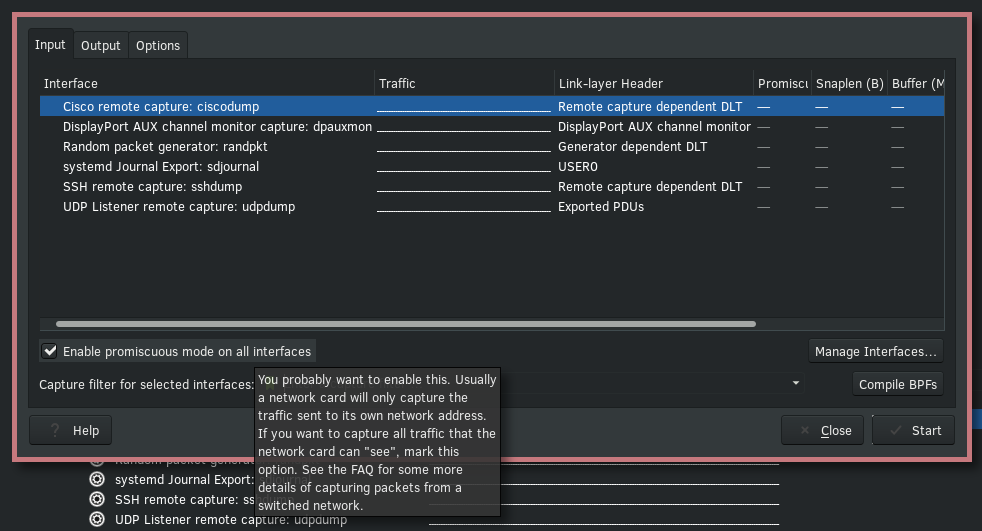
\includegraphics[width=0.618\textwidth]{graphics/capture_options.png}
      \caption{Auswahl der Netzwerkschnittstelle in den Capture-Optionen}
  \end{center}
\end{figure}

Im Optionen-Reiter der Capture-Optionen kann außerdem eingestellt werden, ob die angezeigten Adressen (MAC, Netwerk/IP, Transport) in Namen aufgelöst werden sollen (sofern möglich).\\

Nach der Aufzeichnung im Labor konnten die Daten als Trace-Dateien abgespeichert werden, um später analysiert zu werden. Zur Vereinfachung der Analyse kann man mithilfe von Filtern die Paketliste u.a. auf bestimmte Protokolle einschränken.
Beispielsweise wird mit dem Filter \inlinecode{tcp.port == 80} nur der Verkehr mit den TCP-Portnummern 80 (HTTP) angezeigt.


\subsection{Vierquadrantenkennlinienfeld}
\begin{figure}[H]
  \begin{center}
    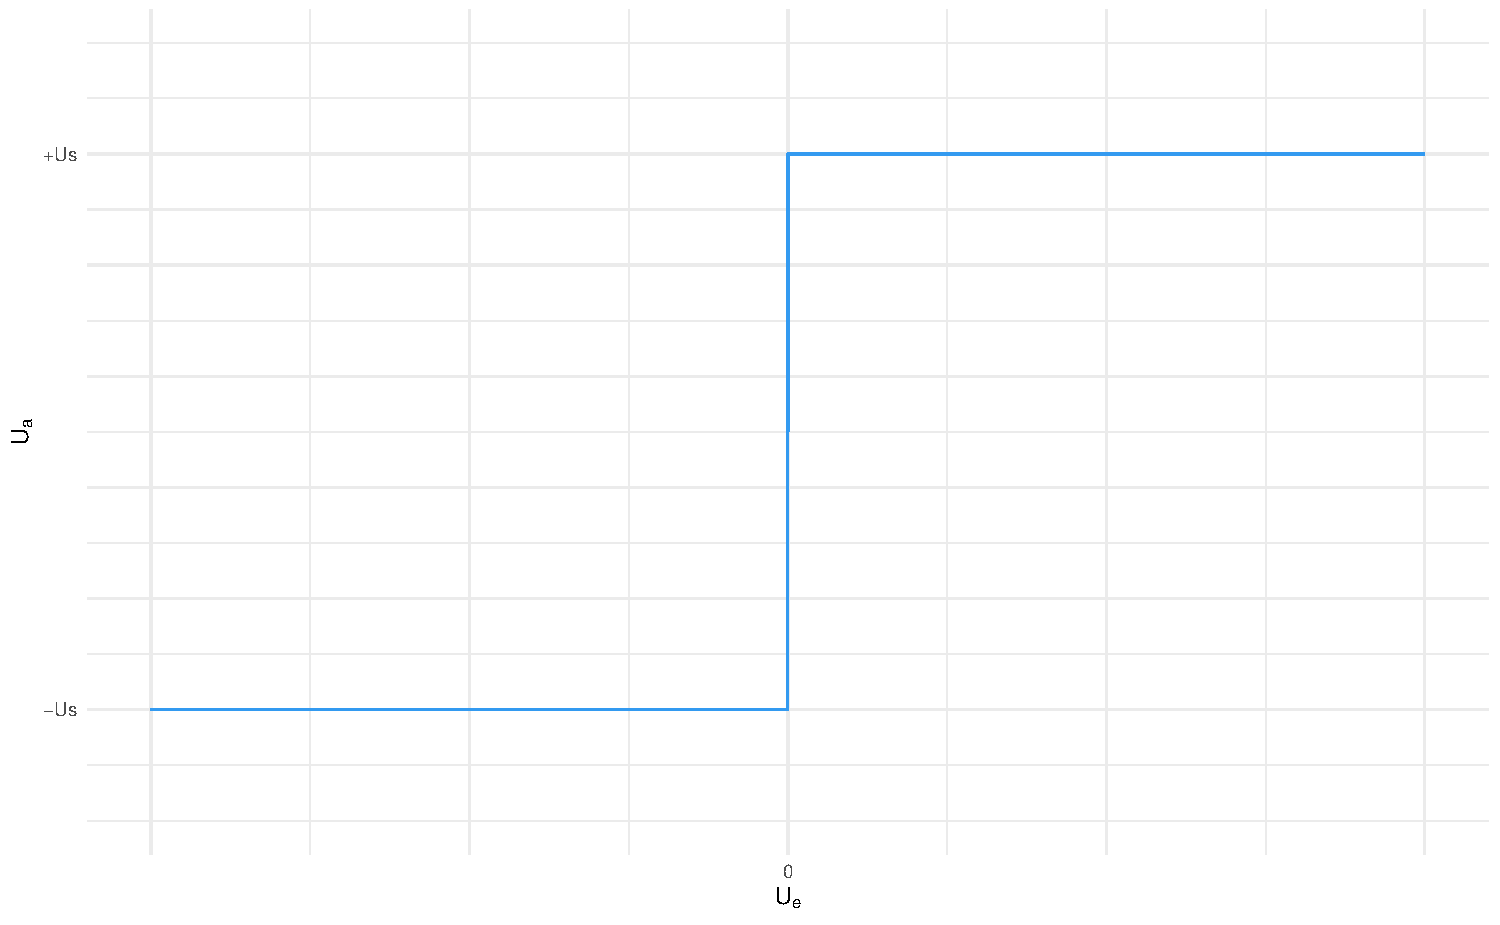
\includegraphics[width=0.618\textwidth]{1_2/opv_nofeed.pdf}
    \end{center}
    \caption{OPV-Kennlinie ohne Rückkopplung (ideal)}
 \end{figure}
\begin{figure}[H]
  \begin{center}
    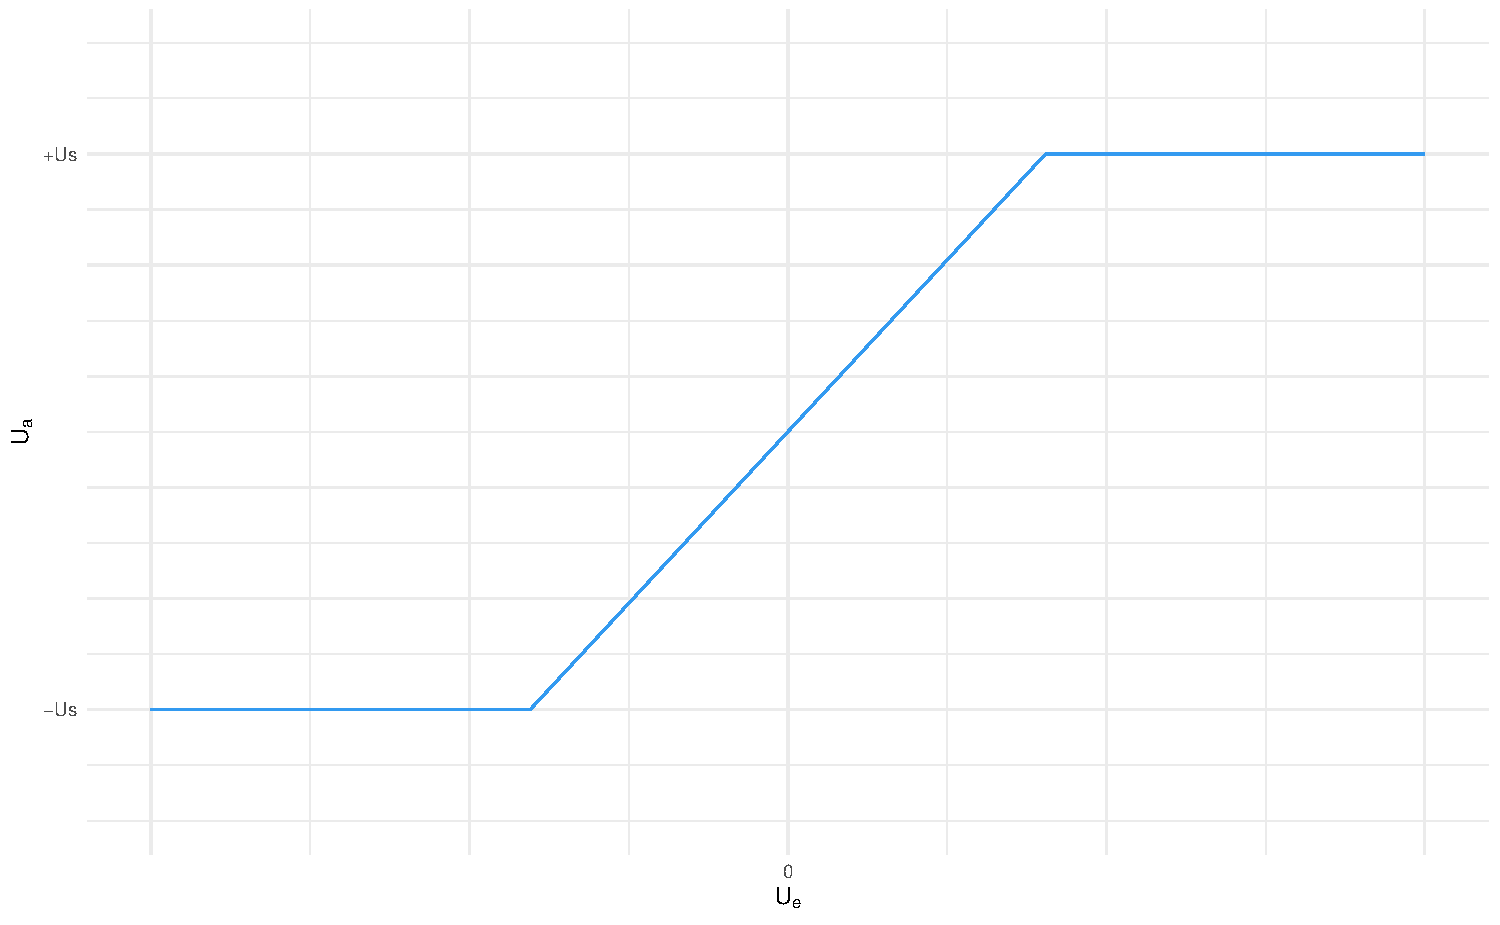
\includegraphics[width=0.618\textwidth]{1_2/opv_feed.pdf}
    \end{center}
    \caption{OPV-Kennlinie mit Rückkopplung}
 \end{figure}

Durch Rückführung eines Teils des Ausgangs- auf das Eingangssignal durch ein
Rückkopplungsnetzwerk wird der Operationsverstärker in einen linearen
Arbeitsbereich gebracht, wodurch die Verstärkung nicht mehr den Wert der der Leerlaufverstärkung (Abb. 1), sondern einen kontrollierten Verstärkungswert (Abb. 2) annimmt.


\subsection{Vierpolersatzschaltbild}
Das Vierpolersatzschaltbild dient zur Kleinsignalbeschreibung des
Bipolartransistors. Die Kapaziäten im physikalischen Ersatzschaltbild führen zu
einer Frequenzabhängigkeit der Vierpolparameter.

\begin{figure}[H]
\begin{center}
\begin{circuitikz}

  \draw (-2,0) to[open, v=$u_1$] (-2,-4);
  \draw (9,0) to[open, v=$u_2$] (9,-4);

  \draw (-2,0) to [short, o-, i=$i_1$] (1,0)
              to [R, l=$h_{11}$] (1,-2)
              to [voltage source, l=$h_{12}\cdot u_2$, v_=$$, -*] (1,-4);

  \draw (5, -4) to[current source, l=$h_{21} \cdot i_1$, i=$$, *-] (5,0);
  \draw (6.618,0) to[R, l=$\dfrac{1}{h_{22}}$, *-*] (6.618, -4);


   \draw (-2,-4) to [short, o-o] (9,-4);
   \draw (5,0) to [short, -o] (9,0);
\end{circuitikz}
\caption{Hybridparametermodell}
\end{center}
\end{figure}
\[h_{11} \vcentcolon= \frac{u_1}{i_1}\rvert_{u_2=0}\]
\[h_{12} \vcentcolon= \frac{u_1}{u_2}\rvert_{i_1=0}\]
\[h_{21} \vcentcolon= \frac{i_2}{i_1}\rvert_{u_2=0}\]
\[h_{22} \vcentcolon= \frac{i_2}{u_2}\rvert_{i_1=0}\]


\begin{figure}[H]

\begin{center}
\begin{circuitikz}

  \draw (-3,0) to[open, v=$u_{BE}$] (-3,-4);
  \draw (9,0) to[open, v=$u_{CE}$] (9,-4);

  \draw (-3,0) to [short, o-, i=$i_1$] (1,0);
  \draw (0, 0) to [R, l_=$r_\pi$, *-*] (0,-4);
  \draw (1.382, 0) to [C, l=$C_{BE}$, *-*] (1.382,-4);

  \draw (1,0) to[C, l=$C_{BC}$] (5,0);

  \draw (5, -4) to[current source, l=$g_m u_{BE}$, i=$$, *-*] (5,0);
  \draw (6.618,0) to[R, l=$r_0$, *-*] (6.618, -4);


   \draw (-3,-4) to [short, o-o] (9,-4);
   \draw (5,0) to [short, -o] (9,0);
\end{circuitikz}
\end{center}
\caption{Kleinsignalersatzschaltbild des Bipolartransistors}
\end{figure}

\noindent Steilheit/Übertragungsleitwert:
\[ g_m = \frac{\dif I_{C}}{\dif U_{BE}} = \frac{I_{C,A}}{U_T} \]
Eingangswiderstand:
\[ r_\pi = \frac{\dif U_{BE}}{\dif I_B} = \frac{\beta_N}{g_m}= \frac{\beta_N \cdot U_T}{I_{C,A}} \]
Ausgangswiderstand ($U_{AN}:$ Early-Spannung):
\[r_0 = \frac{\dif U_{CE}}{\dif I_C} = \frac{U_{AN} + U_{CE,A}}{I_{C,A}}\]

\noindent Rückwärtssteilheit:
\[ \frac{\dif I_B}{\dif U_{CE}} \approx 0\]

\noindent $C_{BC}$: Sperrschichtkapazität (dominiert im normalen Verstärkerbetrieb)
\noindent $C_{BE}$: Diffusionskapaziät \\

\noindent Hybridparameter:

\begin{gather*}
  h_{11} \vcentcolon= \frac{u_1}{i_1}\rvert_{u_2=0}\\
  h_{11} = \frac{r_\pi \cdot \frac{1}{j\omega(C_{BE} + C_{BC})}}{r_\pi + \cdot
    \frac{1}{j\omega(C_{BE} + C_{BC})}} = \frac{r_\pi}{j\omega r_\pi
    (C_{BE}+C_{BC}) + 1}
\end{gather*}

\eqbox{
  h_{11} = r_\pi \cdot \frac{1}{1 + j\omega r_\pi(C_{BE} + C_{BC})}
}{0.618\textwidth}

\begin{gather*}
  h_{12} \vcentcolon= \frac{u_1}{u_2}\rvert_{i_1=0}\\
  i_1=0 \rightarrow i_B = 0 \rightarrow \beta_N \cdot i_B = 0 \rightarrow u_2 =
  0\\
\end{gather*}

\eqbox{
  h_{12} = 0
}{0.618\textwidth}

\begin{gather*}
  h_{21} \vcentcolon= \frac{i_2}{i_1}\rvert_{u_2=0}\\
  i_1 = \frac{u_{BE}}{r_\pi//(\frac{1}{j\omega(C_{BC}+C_{BE})})}\\
  i_2 = i_c = g_m \cdot u_{BE} = \frac{\beta_N}{r_\pi}\cdot u_{BE}\\
  \frac{1}{h_{21}} = \dfrac{\frac{u_{BE}}{\dfrac{r_\pi \cdot
      \frac{1}{j\omega(C_{BC}+C_{BE})}}{r_\pi +
      \frac{1}{j\omega(C_{BC}+C_{BE}}}} } { \dfrac{\beta_N}{r_\pi} \cdot u_{BE}}
 = \dfrac{\frac{1}{\dfrac{
      \frac{1}{j\omega(C_{BC}+C_{BE})}}{r_\pi +
      \frac{1}{j\omega(C_{BC}+C_{BE}}}} } { \beta_N }
 = \dfrac{\dfrac{
     1}{\frac{1}{r_\pi \cdot j\omega(C_{BC}+C_{BE}) + 1}} } { \beta_N }\\
 = \frac{1}{\beta_N \cdot \dfrac{1}{r_\pi \cdot j\omega(C_{BC}+C_{BE})+1}}\\
\end{gather*}
\vspace{-1cm}
\eqbox{
h_{21}=\beta_N \cdot \frac{1}{1 + j\omega r_\pi (C_{BC}+C_{BE})}}{0.618\textwidth}
($\omega \rightarrow 0 \rightarrow h_{21} = \beta_N$ )

\begin{gather*}
  h_{22} \vcentcolon= \frac{i_2}{u_2}\rvert_{i_1=0}\\
  \frac{1}{h_{22}}=r_0//\left(\frac{1}{j\omega C_{BC}} + (r_\pi //
    \frac{1}{j\omega C_{BE}})\right)\\
  = r_0 // \left( \frac{1}{j\omega C_{BC}} + \dfrac{1}{\frac{1}{r_\pi} + j\omega C_{BE}} \right)\\
  = \frac{r_0 \cdot \left( \dfrac{1}{j\omega C_{BC}} + \dfrac{1}{\frac{1}{r_\pi}
        + j\omega C_{BE}} \right)}{ r_0 + \left( \dfrac{1}{j\omega C_{BC}} +
      \dfrac{1}{\frac{1}{r_\pi} + j\omega C_{BE}} \right)}
\end{gather*}

\eqbox{
  \frac{1}{h_{22}} = \dfrac{r_0}{1 + \dfrac{r_0}{\left( \dfrac{1}{j\omega C_{BC}}
        + \dfrac{1}{r_\pi + j\omega C_{BE}} \right)}}
}{0.618\textwidth}

\noindent y-Parameter:
\begin{gather*}
  y_{11}=\frac{1}{h_{11}}\\
  y_{12}=\frac{-h_{12}}{h_{11}}\\
  y_{21}=\frac{h_{21}}{h_{11}}\\
  y_{22}=\frac{\textrm{det} H }{h_{11}}
\end{gather*}

\subsection{Transistorgrundschaltungen}
\begin{figure}[H]
  \begin{center}
    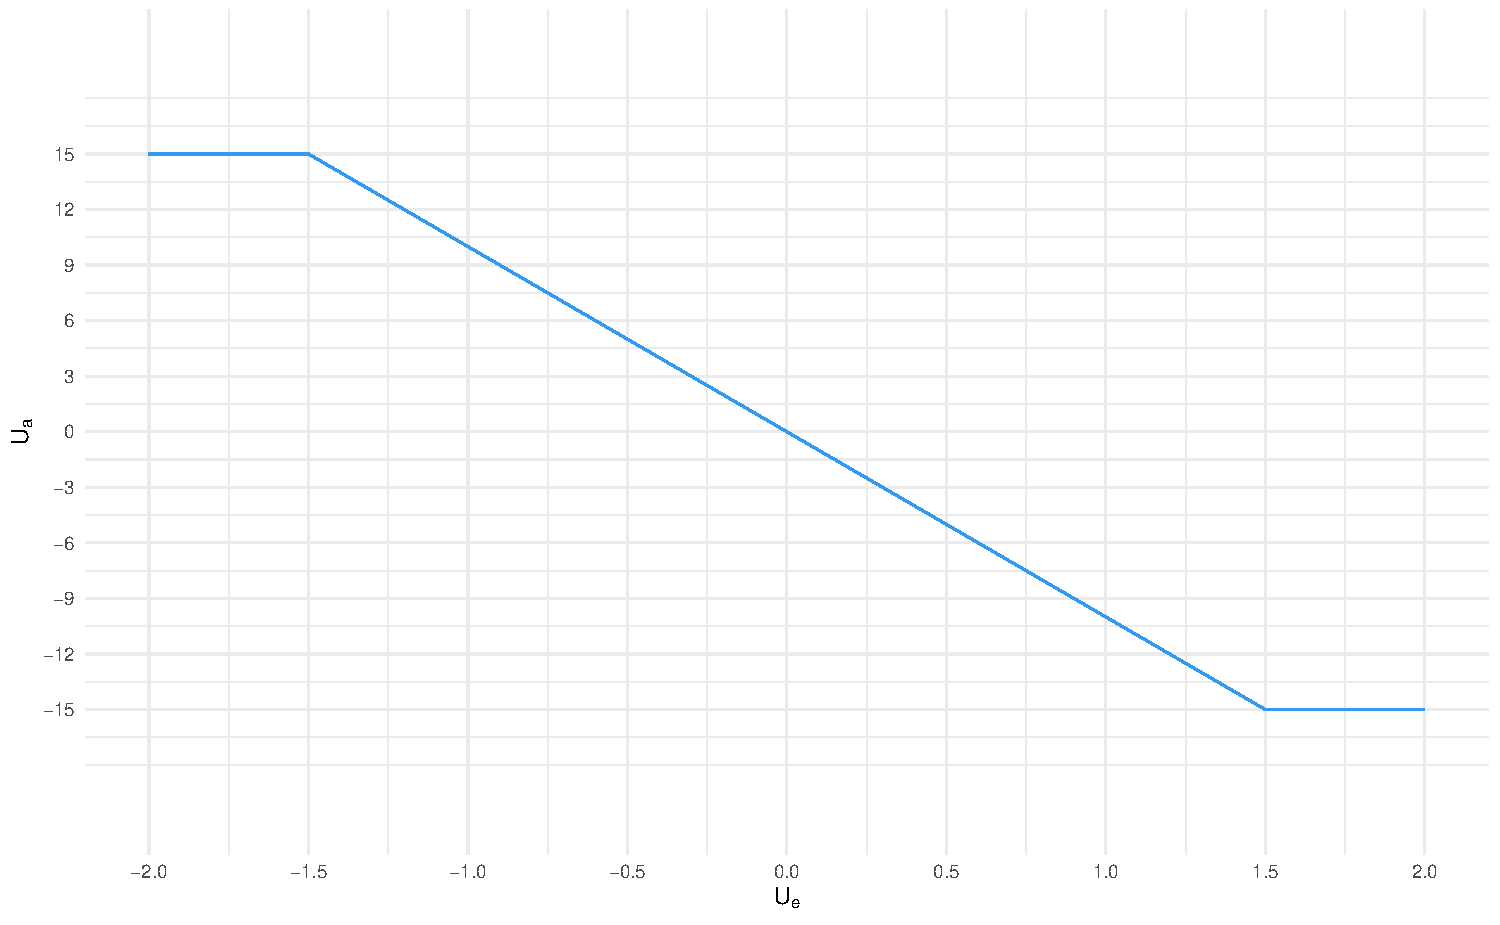
\includegraphics[width=\textwidth]{1_4/opv_inv_verst.pdf}
    \end{center}
    \caption{Kennlinie einer invertierenden OPV-Verstärkerschaltung mit einer Verstärkung von $V_u = -10$ und einer
      Versorgungsspannung von $U_s = \pm 15 \, \si{\volt}$}
 \end{figure}


\subsection{Dimensionierung einer Emitterstufe}
\begin{figure}[H]
  \begin{center}
    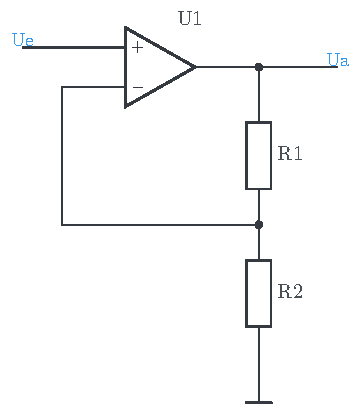
\includegraphics[height=0.618\textwidth]{circuits/nichtinv_verst.pdf}
    \end{center}
    \caption{Nichtinvertierende Verstärkerschaltung}
 \end{figure}

 \begin{gather*}
  U_a = V_0(U_p-U_n)\\
  U_a = V_0(U_e-U_n)\\
  U_n = U_a \frac{R_1}{R_1+R_2}\\
  U_a = V_0 (U_e - U_a \frac{R_1}{R_1 + R_2})\\
  U_a (1 + V_0 \frac{R_1}{R_1 + R_2}) = V_0 U_e\\
  \frac{U_a}{U_e} = V = \frac{V_0}{1 + V_0 \frac{R_1}{R_1+R_2}}\\
  \intertext{für $V_0 \rightarrow \infty$}
  V = \frac{R_1 + R_2}{R_1} = 1 + \frac{R_2}{R_1}
\end{gather*}



\subsection{Temperaturabhängigkeiten}
Temperaturänderungen stellen für den Transistor als Halbleiterbauelement eine
externe Energiezufuhr und damit eine Störung des thermodynamischen
Gleichgewichts dar. Die Ladungsträgerdichten der einzelnen Bereiche
erhöhen sich, die Weiten der Raumladungszonen verringern sich und der Transistor
wird insgesamt leitfähiger. Dadurch erhöht sich auch der
Stromverstärkungsfaktor $\beta$, was z.B. den Arbeitspunkt, der bei der
Schaltungsdimensionierung angenommen wurde, verschieben kann. Da dieser zusätzlich
fertigungsbedingt abweichen kann, strebt man einen
Arbeitspunkt an, der möglichst unabhängig von der Stromverstärkung ist. Dies
wird z.B. durch die Arbeitspunkteinstellung mit einem 4-Widerstandsnetzwerk mit Stromgegenkopplung oder die Einstellung des Emitterstroms durch eine Stromquelle erreicht.



\subsection{Bestimmung der Grundschaltungsparameter}
Die Parameter werden nach dem physikalischen Ersatzschaltbild des
Bipolartransistors ohne parasitäre Kapazitäten bestimmt. Bei der
Kleinsignalanalyse werden alle Kapazitäten sowie Spannungsquellen als
Kurzschlüsse behandelt.

\subsubsection{Emitterschaltung}

\begin{figure}[H]
  \begin{center}
    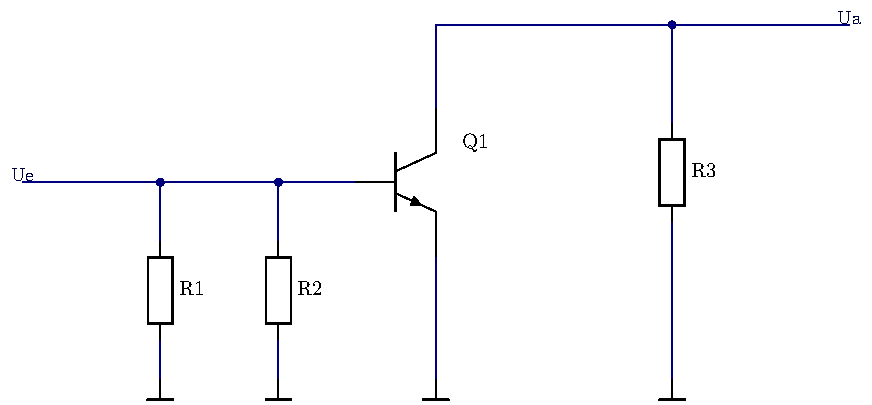
\includegraphics[width=0.618\textwidth]{circuits/commonEmitter_ESB1.pdf}
  \end{center}
  \caption{Kleinsignalersatzschaltbild der Emitterschaltung (Abb. 3)}
\end{figure}

\begin{figure}[H]
  \begin{center}
    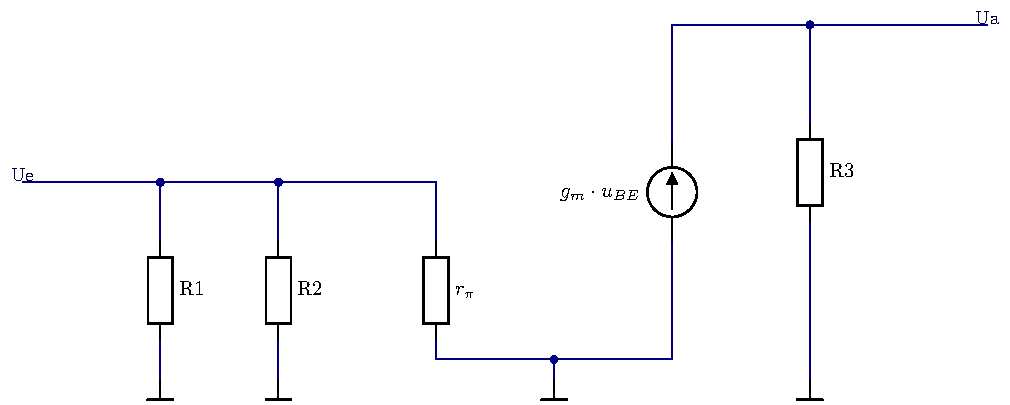
\includegraphics[width=0.618\textwidth]{circuits/commonEmitter_ESB2.pdf}
  \end{center}
  \caption{ESB Abb. 6, Transistor durch phys. ESB ersetzt}
\end{figure}

\noindent Eingangswiderstand:
\[r_e = \frac{U_e}{I_e} = R_1 // R_2 // r_\pi\]
\noindent Ausgangswiderstand:
\[r_a = \frac{U_a}{I_a} = r_0 // R_3 \]
\noindent Spannungsverstärkung:
\[V_u = \frac{U_2}{U_1}\]

\begin{gather*}
  U_2 = g_m \cdot u_{BE} \cdot (r_0 // R_3) = g_m \cdot U_1 \cdot (r_0 // R_3)\\
  V_u = g_m \cdot (r_0 // R_3)
\end{gather*}

\noindent Stromverstärkung:
\[V_i = \frac{I_2}{I_1}\]
\[I_1 = \frac{U_1}{r_\pi} + U_1 (\frac{1}{R_2} + \frac{1}{R_1})\]
\[I_B = \frac{U_1}{r_\pi} = I_1 - U_1 (\frac{1}{R_2} + \frac{1}{R_1})\]
\[I_2 = g_m \cdot U_1 \rightarrow U_1 = \frac{I_2}{g_m}\]
\[ \frac{I_2}{g_m \cdot r_\pi}  = I_1 - \frac{I_2}{g_m} (\frac{1}{R_2} + \frac{1}{R_1}) \]
\[ \frac{1}{g_m \cdot r_\pi}  = \frac{I_1}{I_2} - \frac{1}{g_m} (\frac{1}{R_2} + \frac{1}{R_1}) \]
\[\frac{I_2}{I_1} = V_i = \frac{1}{ \frac{1}{g_m} (\frac{1}{r_\pi} +
    \frac{1}{R_2} + \frac{1}{R_1}) }\]

\noindent Leistungsverstärkung:
\[V_p = \frac{P_2}{P_1} = \frac{U_2 \cdot I_2}{U_1 \cdot I_1} = V_u \cdot V_i\]
\[V_p = \frac{g_m^2 \cdot (r_0 // R_3)}{\frac{1}{r_{\pi}} + \frac{1}{R_2} + \frac{1}{R_1}}\]

%%%%%%%%%%%%%%%%%%%%%%%%%%%%%%%%%%%%%%%%%
\subsubsection{Kollektorschaltung}
\begin{figure}[H]
  \begin{center}
    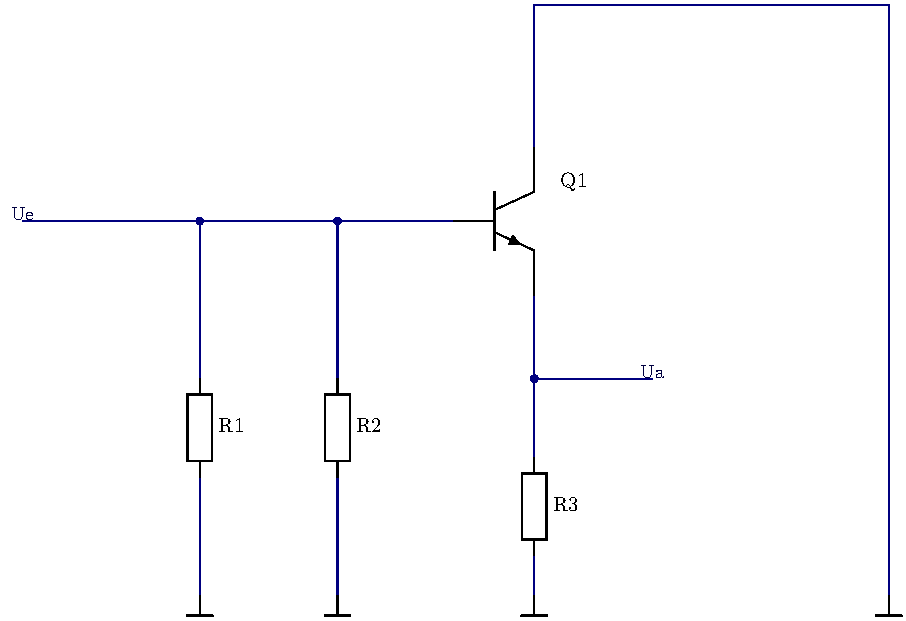
\includegraphics[width=0.618\textwidth]{circuits/commonCollector_ESB1.pdf}
  \end{center}
  \caption{Kleinsignalersatzschaltbild der Kollektorschaltung (Abb. 4)}
\end{figure}


\begin{figure}[H]
  \begin{center}
   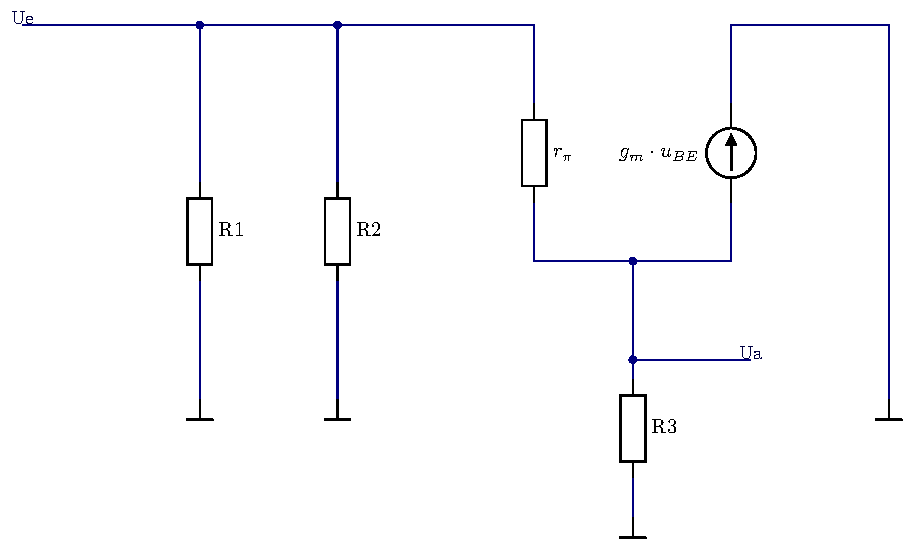
\includegraphics[width=0.618\textwidth]{circuits/commonCollector_ESB2.pdf}
  \end{center}
  \caption{ESB Abb. 8, Transistor durch phys. ESB ersetzt}
\end{figure}
\noindent Eingangswiderstand
\[ r_e = \frac{U_1}{I_1}\]
\[ r_e = R_1 // R_2 // (r_\pi + \beta_N R_3)\]

\noindent Ausgangswiderstand
\[ r_a = \frac{U_2}{I_2}|_{U_1 = 0}\]
\[U_2 = U_{BE}\]
\[r_a = R_3 // \frac{r_\pi }{\beta_N + 1}\]
\[r_a \approx \frac{1}{g_m}\]

\noindent Spannungsverstärkung
\[ V_u = \frac{U_2}{U_1}\]
\[V_u = \frac{1}{1+ \dfrac{1}{g_m \cdot R_3}} \approx 1\]

%%%%%%%%%%%%%%%%%%%%%%%%%%%%%%%%%%%%%%%%%
\subsubsection{Basisschaltung}
\begin{figure}[H]
  \begin{center}
    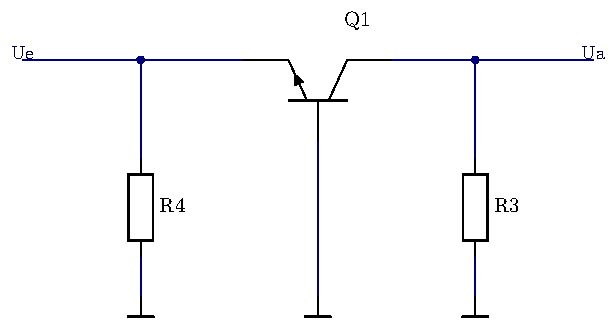
\includegraphics[width=0.618\textwidth]{circuits/commonBase_ESB1.pdf}
  \end{center}
  \caption{Kleinsignalersatzschaltbild der Basisschaltung (Abb. 5)}
\end{figure}

\begin{figure}[H]
  \begin{center}
    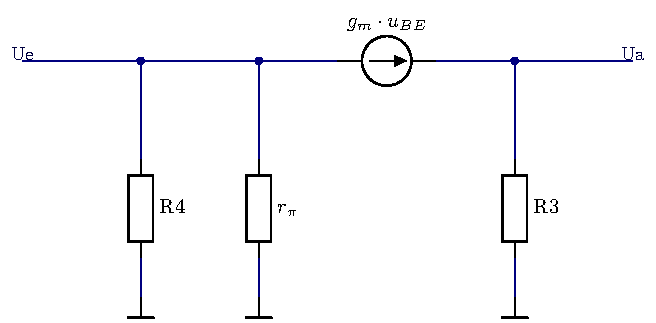
\includegraphics[width=0.618\textwidth]{circuits/commonBase_ESB2.pdf}
  \end{center}
  \caption{ESB Abb. 10, Transistor durch phys. ESB ersetzt}
\end{figure}

\noindent Eingangswiderstand
\[ r_e = \frac{U_1}{I_1}\]
\[0 = I_1 + \frac{U_1}{R_4} + \frac{U_1}{r_\pi} + g_m U_{BE} \]
\[I_1 = - \frac{U_1}{R_4} - \frac{U_{BE}}{r_\pi} - g_m U_{BE} \]
\[U_{BE} = - U_1\]
\[I_1 = \frac{U_1}{R_4} + \frac{U_1}{r_\pi} + g_m U_{1} \]
\[ \frac{I_1}{U_1} = \frac{1}{R_4} + \frac{1}{r_\pi} + g_m \]
\[ r_e = \frac{1}{ \frac{1}{R_4} + \frac{1}{r_\pi} + g_m} \]
\[g_m = \frac{B_n}{r_\pi}\]
\[ r_e = \frac{1}{\frac{1}{R_4} + \frac{1}{r_\pi} (1+B_N)} \]
\[ r_e = \frac{1}{R_4} // (r_\pi (\frac{1}{1+B_N}))\]

\noindent Ausgangswiderstand
\[ r_a = \frac{U_2}{I_2}|_{U_e = 0}\]
\[ I_2 = g_m U_{BE} + \frac{U_2}{R_3 // r_0}\]
\[ U_{BE} = 0\]
\[ r_a = R_3 // r_0\]

\noindent Spannungsverstärkung
\[V_u = \frac{U_2}{U_1}\]
\[U_2 = -g_m \cdot U_{BE} (R_3 // r_0)\]
\[U_{BE} = - U_{1}\]
\[ \frac{U_2}{U_1} = V_u = g_m (R_3 // r_0)\]

\subsection{Messtechnische Bestimmung der Ein- und Ausgangsparameter}
\subsubsection{Bestimmung des Eingangswiderstands}
Allgemein gelingt die Widerstandsmessung indirekt durch eine Spannungs- und
Strommessung und anschließende Division der gemessenen Größen. 

\subsubsection{Bestimmung des Ausgangswiderstands}
Der Zusammenhang zwischen Lastwiderstand und Ausgangswiderstand des Verstärkers
ist linear (Zweipol)
\[R_a = \frac{U_{a,0} - U_{a,Last}}{I_{a,Last}}\]
\[R_a = \frac{U_{a,0} - U_{a,Last}}{U_{a,Last}} \cdot R_L\]
\[R_a = R_L \cdot \left(\frac{U_{a,0}}{U_{a,Last}}-1 \right)\]

Wobei $U_{a,0}$ die Leerlaufspannung am Ausgang, $U_{a,Last}$ die
Spannung am Ausgang bei Belastung mit dem Lastwiderstand $R_L$, und $R_a$ der
Ausgangswiderstand des Verstärkers ist.

Aus der Gleichung lässt sich erkennen, dass $R_a = R_L$ wenn $U_{a,Last} =
U_{a,0}/2$ ist. D.h. die Ausgangsspannung $U_{a,Last}$ kann bei
Belastung mit einem bekannten Lastwiderstandswert gemessen und anschließend in
der obigen Gleichung verwendet werden oder sie kann auf den halben Wert der
Leerlaufausgangsspannung durch einen variablen Lastwiderstand eingestellt
werden, wonach eine Messung des Lastwiderstandes folgt.


\subsubsection{Bestimmung der Verstärkungen}
Da die Verstärkungen frequenzabhängig sind und somit das Verhältnis von Ein- und
Ausgangsspannung (wechselspannungsmäßig) nicht konstant ist, muss man messtechnisch die
Übertragungsfunktion ermitteln, was beispielsweise durch das Durchlaufen mehrerer
Signalfrequenzen und anschließender Darstellung der
Ausgangsamplituden/-differenz erreicht werden kann (wobbeln). 

\subsection{Bootstrapschaltung}
\subsubsection{Differenzverstärker}

\begin{figure}[H]
  \begin{center}
    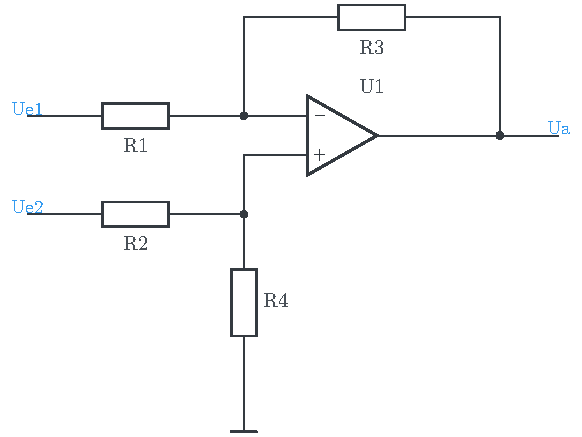
\includegraphics[width=0.618\textwidth]{circuits/differenz.pdf}
  \end{center}
  \caption{Differenzverstärkerschaltung}
\end{figure}

Der Differenzverstärker verstärkt die Differenz der Spannungen $U_{e1}$ und $U_{e2}$.

\begin{gather*}
  \intertext{Überlagerung:}
  U_a = U_a' + U_a''\\
  U_a' = U_a|_{U_{e2} = 0} = - U_{e1} \cdot \frac{R_3}{R_1}\\
  U_a'' = U_a|_{U_{e1} = 0} = U_p \cdot \left(1+\frac{R_3}{R_1}\right)\\
  = U_{e2}  \frac{R_4}{R_2 + R_4} \cdot \left(1+\frac{R_3}{R_1}\right)\\
  U_a = U_{e2}  \cdot \frac{R_4}{R_2 + R_4} \cdot \left(1+\frac{R_3}{R_1}\right) -
  U_{e1} \cdot \frac{R_3}{R_1}\\
  U_a = U_{e2}  \cdot \frac{R_4}{R_2 + R_4} + U_{e2} \cdot \frac{R_4}{R_2 + R_4}
  \cdot \frac{R_3}{R_1} - U_{e1} \cdot \frac{R_3}{R_1}
\end{gather*}
\noindent Wenn gilt $\frac{R_3}{R_1} = \frac{R_4}{R_2}:$
\eqbox{
  U_a = \frac{R_3}{R_1}\left(U_{e2} - U_{e1}\right)
}{0.382\textwidth}

\noindent Wenn alle Widerstände gleich dimensioniert werden:
\eqbox{
  U_a = U_{e2} - U_{e1}
}{0.382\textwidth}


\subsubsection{Instrumentationsverstärker}

\begin{figure}[H]
  \begin{center}
    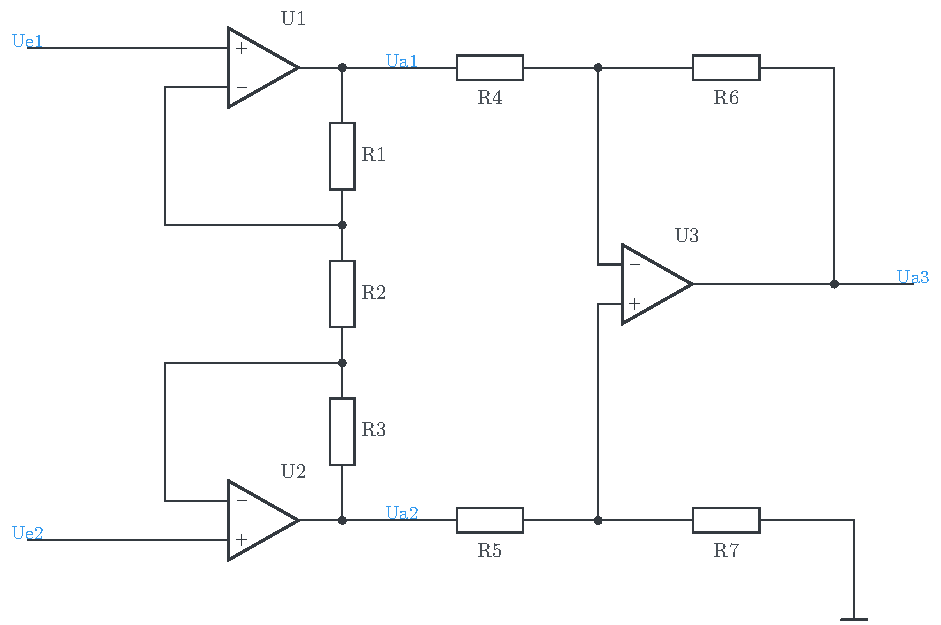
\includegraphics[height=0.618\textwidth]{circuits/instrument.pdf}
  \end{center}
  \caption{Instrumentationsverstärkerschaltung}
\end{figure}

\begin{gather*}
  \intertext{Virtuelle Masse, $U_d = 0$:}
  U_{R_2} = U_{e1} - U_{e2}\\
  I_{R_2} = \frac{U_{e1} - U_{e2}}{R_2}\\
  \intertext{für $I_n = 0$:}
  I_{R_1} = I_{R_2} = I_{R_3}\\
  U_{a1,2} = U_{a1} - U_{a2} = I_{R_3} (R_1 + R_2 + R_3)\\ 
  U_{a1} - U_{a2} = \frac{U_{e1}-U_{e2}}{R_2} (R_1 + R_2 + R_3)\\ 
  \intertext{für $R_1 = R_3$:}
  U_{a1} - U_{a2} = U_{e1} - U_{e2} \left( 1 + \frac{2 \cdot R_1}{R_2}\right)
\end{gather*}
  der Dritte OPV ist als Differenzverstärker geschaltet\\
  für $R_4 = R_5 = R_6 = R_7$ ist die Verstärkung $V_{OPV3} = -1$
    (Eingangsdifferenz tauschen)

\eqbox{
  U_{a3} = (U_{e2} - U_{e1}) \cdot (1 + \frac{2\cdot R_1}{R_2})
}{0.618\textwidth}
Die Verstärkung ist somit durch $R_2$ einstellbar
\subsubsection{Summierer}

\begin{figure}[H]
  \begin{center}
    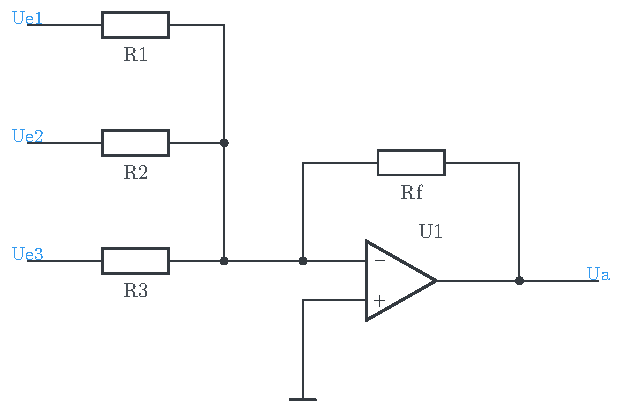
\includegraphics[width=0.618\textwidth]{circuits/summier.pdf}
  \end{center}
  \caption{Summierverstärkerschaltung}
\end{figure}

Der Summierverstärker verstärkt die Summe der gewichteten Eingangsspannungen.

\begin{gather*}
  I_{\mathrm{IN}} = \sum_{n=1}^N{I_{en}} = \frac{U_{e1}}{R_1}+
  \frac{U_{e2}}{R_2} + \cdots + \frac{U_{eN}}{R_N}\\
\end{gather*}
\eqbox{
  U_a = -\left( \frac{R_f}{R_1} U_{e1} + \frac{R_f}{R_2} U_{e2} + \cdots +
    \frac{R_f}{R_N} U_{eN} \right)
  }{0.618\textwidth+5mm}

\subsubsection{Integrator}
\begin{figure}[H]
  \begin{center}
    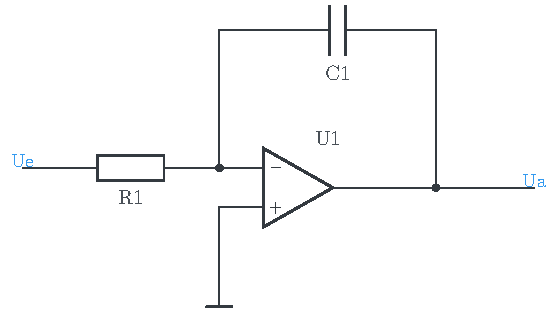
\includegraphics[width=0.618\textwidth]{circuits/integrier.pdf}
  \end{center}
  \caption{Integratorschaltung}
\end{figure}

\begin{gather*}
i_{R_1} = - i_{C_1}\\
\frac{u_e}{R_1} = - C_1 \cdot \frac{\dif u_a}{\dif t}
\end{gather*}
\eqbox{
u_a = - \frac{1}{R_1 C_1} \cdot \int{u_e \dif t}
}{0.382\textwidth}
Der Integrator bildet also das Integral der Eingangsspannung, wichtet es mit
$\frac{1}{RC}$ ($RC...\mathrm{Zeitkonstante}$) und invertiert es.

\subsubsection{Differentiator}
\begin{figure}[H]
  \begin{center}
    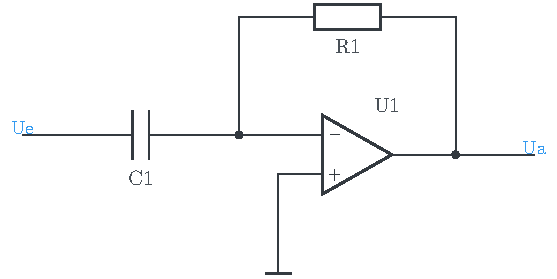
\includegraphics[width=0.618\textwidth]{circuits/differenzier.pdf}
  \end{center}
  \caption{Differentiatorschaltung}
\end{figure}

\begin{gather*}
i_{R_1} = - i_{C_1}\\
\frac{u_a}{R_1} = - C_1 \cdot \frac{\dif u_e}{\dif t}
\end{gather*}
\eqbox{
u_a = - {R_1 C_1} \cdot \frac{\dif u_e}{\dif t}
}{0.382\textwidth}
Der Differentiator differenziert die Eingangsspannung, wichtet das Ergebnis mit
$RC$ und invertiert es.


\subsection{Frequenzverhalten}
Das Frequenzverhalten des Bipolartransistors wird durch die
Sperrschichtkapazität $C_{BC}$, welche im Normalbetrieb dominiert, sowie die
Diffusionskapazität $C_{BE}$ bestimmt, da diese im Ersatzschaltbild
frequenzabhängige Widerstände darstellen. 

\subsection{Grenzfrequenz und Bandbreite}
Man kann den Betrag der Stromverstärkung $\beta$ des Bipolartransistors über der
Frequenz (z.B. im Bode-Diagramm) auftragen. Der Einfluss der parasitären
Kapazitäten resultiert in einem tiefpassartigen Verlauf der Stromverstärkung.
Markante Punkte sind die Grenzfrequenz, bei welcher die Verstärkung um den
Faktor $\frac{1}{\sqrt{2}}$ (halbierte Leistung) fällt, sowie die
Transitfrequenz, bei welcher der Betrag der Verstärkung gleich eins ist.

Die Bandbreite beschreibt die Differenz zwischen der maximalen und der
minimalen Frequenz, die eine Dämpfung der Stromverstärkung um
$\frac{1}{\sqrt{2}}$ aufweisen (obere und untere Grenzfrequenz).

\subsection{Millertheorem}
Das Millertheorem besagt, dass sich eine zwischen Ein- und Ausgangskreis
befindliche Impedanz durch zwei separate, jeweils im Ein- und Ausgangskreis
befindliche, Impedanzen ersetzen lässt. Dies ist bei der Analyse des
Kleinsignalersatzschaltbildes mit parasitären Kapazitäten (Abb. 2) hilfreich, da dort die
Sperrschichtkapazität $C_{BC}$ den Ausgangskreis mit dem Eingangskreis koppelt.
Sie lässt sich in zwei resultierende Miller-Kapazitäten transformieren.
\[I_1 = \frac{U_1 - U_2}{Z} = \frac{U_1 - V_u \cdot U_1}{Z} = \frac{U_1
    (1-V_u)}{Z} = \frac{U_1}{ \underbrace{\frac{Z}{1-V_u}}_{Z'} }\]
\[Z' = \frac{Z}{1-V_u}\]
\noindent analog gilt für die ausgangsseitige Impedanz
\[Z'' = \frac{Z}{1- \frac{1}{V_u} }\]

\noindent setzt man
\[Z = \frac{1}{j \omega C_{BC}}\]
\noindent für die Sperrschichtmillerkapazitäten, erhält man
\[C_{BC}' = C_{BC}(1-V_u)\]
\[C_{BC}'' = C_{BC}(1-\frac{1}{V_u})\]


\subsection{Grenzfrequenz der Emitterschaltung}
\begin{figure}[H]
  \begin{center}
    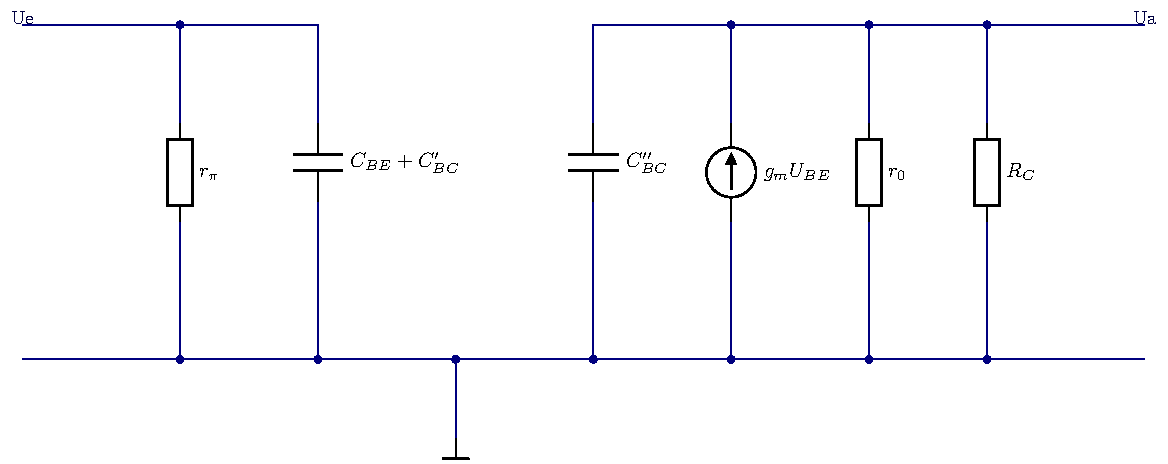
\includegraphics[width=0.618\textwidth]{circuits/commonEmitter_freq.pdf}
  \end{center}
  \caption{ESB der Emitterschaltung mit Millerkapazitäten}
\end{figure}

Die obere Grenzfrequenz der Schaltung wird durch die parasitären Kapazitäten des
Bipolartransistors bestimmt, die untere durch die Koppelkondensatoren der Schaltung

Eingangskreis:
\[0 = \frac{U_1}{r_\pi} + U_1 j \omega (C'_{BC}+C_{BE})-I_b\]

\noindent Ausgangskreis:
\[0 = g_m U_1 + \frac{U_a}{r_0 // R_C} - U_a j \omega C_{BC}''\]

\noindent Übertragungsfunktion
\[\frac{U_a}{U_e} = \frac{\frac{1}{r_\pi} +
    j\omega(C_{BC}'+C_{BE}) -g_m}{\frac{1}{r_0 // R_C} - j\omega C_{BC}''}\]

\noindent Grenzfrequenz
\[\omega_{gr} = \frac{1}{(C_{BE}+C_{BC}')r_\pi }\]

\[\left( \omega_{gr} = \frac{1}{(C_{BC}' + C_{BE})\cdot \frac{1}{g_m} - r_0
      C_{BC}''} \right) ? \]

% 2
%%%%%%%%%%%%%%%%%%%%%%%%%%%%%%%%%%%%%
  
\includepdf{./titlepage/titlepage2.pdf}
  \clearpage
  \setcounter{page}{1}
%%%%%%%%%%%%%%%%%%%%%%%%%%%%%%%%%%%%%

\section{Versuchsaufgaben} 

\setcounter{subsection}{1}
\subsection{Arbeitspunktbestimmung}
Die Ströme und Spannungen konnten teilweise nur indirekt gemessen werden und
mussten daher aus mehreren Messungen berechnet werden.

\subsubsection{ES\_IGK1}
Der Kollektorstrom $I_C$ der Schaltung wurde durch die Messung der Spannung über dem
Widerstand $R_3$ ($V_2 - U_C$)und entsprechender Division durch dessen Widerstandswert
ermittelt.
\[I_C  = \frac{V_2 - U_c}{R_3} = \frac{12.01 \, \si{\volt} - 6.38 \,
    \si{\volt}}{1.3 \, \si{\kilo\ohm}} = 4.33 \, \si{\milli\ampere}\]

Die Kollektorspannung konnte dann über Messung des Emitterpotentials $U_E$ gegen Masse
und Differenzbildung mit dem vorher bestimmten Wert $U_c$ bestimmt werden.
\[U_{CE} = U_C - U_E = 6.38 \, \si{\volt} - 0.436 \, \si{\volt} = 5.944 \, \si{\volt}\]

Der Basisstrom ist die Differenz aus dem Strom durch $R_1$ und dem Strom durch
$R_2$.
\[I_B = \frac{V_2 - U_B}{R_1}-\frac{U_B}{R_2} = \frac{12 \, \si{\volt} - 1.149
    \, \si{\volt}}{43 \, \si{\kilo\ohm}} - \frac{1.149 \, \si{\volt}}{5.1 \,
    \si{\kilo\ohm}} = 27.58 \, \si{\micro\ampere}\]

Die statische Stromverstärkung ist damit
\[B = \frac{I_C}{I_B} = \frac{4.33 \, \si{\milli\ampere}}{27.58 \,
    \si{micro\ampere}} = 157\]

Aus dem Datenblatt des 2N3904 Bipolartransistors lässt sich bei einem
Kollektorstrom vom etwa $I_C = 4 \, \si{\milli\ampere}$ und einer
Kollektor-Emitter-Spannung von $U_{CE} = 10 \, \si{\volt}$ ein
Stromverstärkungsfaktor von $B = 150$ ablesen. (Datenblatt onsemi Abb. 11).

\begin{figure}[H]
  \begin{center}
    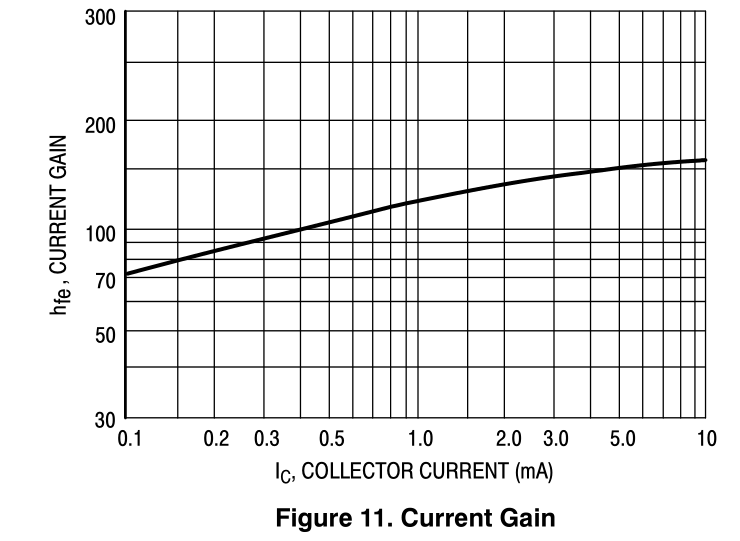
\includegraphics[width=0.618\textwidth]{2_2/ds1}
  \end{center}
  \caption{Quelle: http://onsemi.com}
\end{figure}

\subsubsection{ES\_IUGK1}
Die Arbeitspunktwerte der zweiten und dritten Schaltung wurden entsprechend 2.2.1 bestimmt.

\begin{table}[H]
\begin{center}
\begin{tabular}{c | c}
  $U_C$ & $6.06 \, \si{\volt}$\\
  \hline
  $U_E$ & $0.53 \, \si{\volt}$\\
  \hline
  $U_B$ & $1.23 \, \si{\volt}$\\
\end{tabular}
\end{center}
\caption{Zwischenwerte der Schaltung ES\_IUGK1}
\end{table}

\begin{table}[H]
\begin{center}
\begin{tabular}{c | c}
  $I_C$ & $5.23 \, \si{\milli\ampere}$\\
  \hline
  $U_{CE}$ & $5.53 \, \si{\volt}$\\
  \hline
  $I_{B}$ & $24.15 \, \si{\micro\ampere}$\\
  \hline
  $B$ & $216 $\\
\end{tabular}
\caption{Arbeitspunktwerte der Schaltung ES\_IUGK1}
\end{center}
\end{table}

\subsubsection{KS\_BOS1}

\begin{table}[H]
\begin{center}
\begin{tabular}{c | c}
  $U_C$ & $12.01 \, \si{\volt}$\\
  \hline
  $U_E$ & $4.37 \, \si{\volt}$\\
  \hline
  $U_B$ & $5 \, \si{\volt}$\\
  \hline
  $U_{R1}$ & $6.9 \, \si{\volt}$\\
  \hline
  $U_{R3}$ & $0.63 \, \si{\volt}$\\
\end{tabular}
\end{center}
\caption{Zwischenwerte der Schaltung KS\_BOS1}
\end{table}

\begin{table}[H]
\begin{center}
\begin{tabular}{c | c}
  $I_C$ & $ 1.45 \, \si{\milli\ampere}$\\
  \hline
  $U_{CE}$ & $ 7.91 \, \si{\volt}$\\
  \hline
  $I_{B}$ & $ 4.26 \, \si{\micro\ampere}$\\
  \hline
  $B$ & $340.38$\\
\end{tabular}
\caption{Arbeitspunktwerte der Schaltung KS\_BOS1}
\end{center}
\end{table}



\subsection{Emitterschaltung mit Stromgegenkopplung: ES\_IGK1}
\subsubsection{Spannungsverstärkung}
Die Werte zur Bestimmung der Spannungsverstärkungen wurden bei einer
Eingangsspannung von $U_{\mathrm{RMS}} = 5 \, \si{\milli\volt}$ und einer
Frequenz von $f_e = 1 \, \si{\kilo\hertz}$ bestimmt. Der Lastwiderstand wurde
von $100 \, \si{\kilo\ohm}$ bis $1 \, \si{\kilo\ohm}$ variiert. Die
Spannungsverstärkungen bei den jeweiligen Lastwiderstandswerten ist dann
der Quotient aus Ausgangs- und Eingangsspannung. Die Spannungswerte wurden
als RMS-Werte am Oszilloskop gemessen. Der interne Lastwiderstand beträgt $R_{\mathrm{L,intern}} =
100 \, \si{\kilo\ohm}$.

\begin{table}[H]
  \begin{center}
    \begin{tabular}{|c|c|c|c|}
      \hline
      $U_e / \si{\milli\volt}$ & $U_a / \si{\milli\volt}$ & $R_{\mathrm{L,gesamt}} / \si{\kilo\ohm}$ & $V_u$\\
      \hline
      \hline

      4.99 & 810.96 & 100 & 162.5\\
      4.97 & 790.5 & 33.33 & 159.1\\
      4.98 & 721.6 & 9.09 & 144.90\\
      4.97 & 363.9 & 0.99 & 73.22\\
      \hline
    \end{tabular}

  \end{center}

  \caption{RMS-Spannungswerte und daraus resultierende Verstärkung bei
    verscheidenen Lastwiderständen}

\end{table}

\begin{figure}[H]
  \begin{center}
    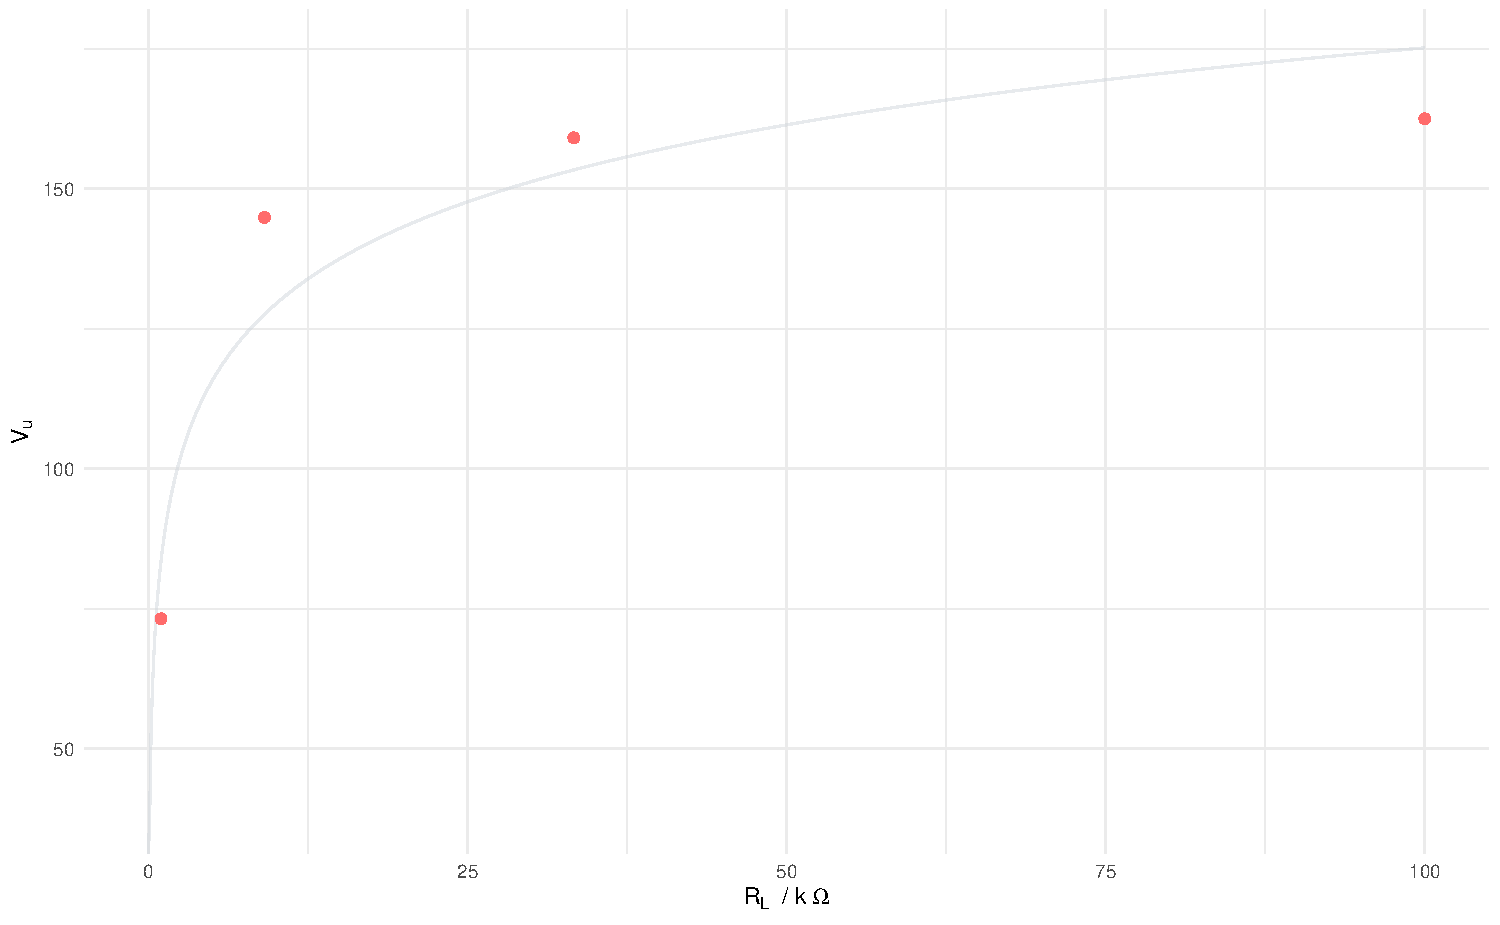
\includegraphics[width=\textwidth]{2_3/2_3_1.pdf}
  \end{center}
  \caption{Graph der Messwerte}
\end{figure}

Der Anstieg des Graphen entspricht der Steilheit $g_m$ des Transistors. Die
Steilheit im Arbeitspunkt ist etwa
\[g_m = \frac{I_C}{U_T} = \frac{4.33 \, \si{\milli\ampere}}{26 \,
    \si{\milli\volt}} = 166.53 \, \si{\milli\siemens}\]

Der theoretische Zusammenhang ist
\[V_u = - g_m \cdot R_L \] 

Der scheinbar lineare Zusammenhang ist aus dem Messwertgraphen jedoch nicht
erkennbar. Dies liegt daran, dass der interne Kollektorwiderstand $R_3$ als
Parallelschaltung in den Gesamtlastwiderstand eingeht.
\[V_u = -g_m \cdot R_3 // R_{\mathrm{L,extern}}\]

$R_3 = 1.3 \, \si{\kilo\ohm}$ legt hier durch die Parallelschaltung den
theoretischen Grenzwert der Spannungsverstärkung fest. \[|V_{u,max}| = 188.26 \,
  \si{\milli\siemens} \cdot 1.3 \, \si{\kilo\ohm} \approx 245\]


Bei hohen externen Widerstandswerten dominiert der Widerstand $R_3$ in der
Parallelschaltung, wodurch der Gesamtlastwiderstand etwa $R_3$ ist, die
Verstärkung läuft gegen einen konstanten Wert.
Bei geringen Widerstandswerten muss die Parallelschaltung berücksichtigt
werden.

Durch Berücksichtung des Kollektorwiderstandes erhält man dann den erwarteten Zusammenhang.

\begin{figure}[H]
  \begin{center}
    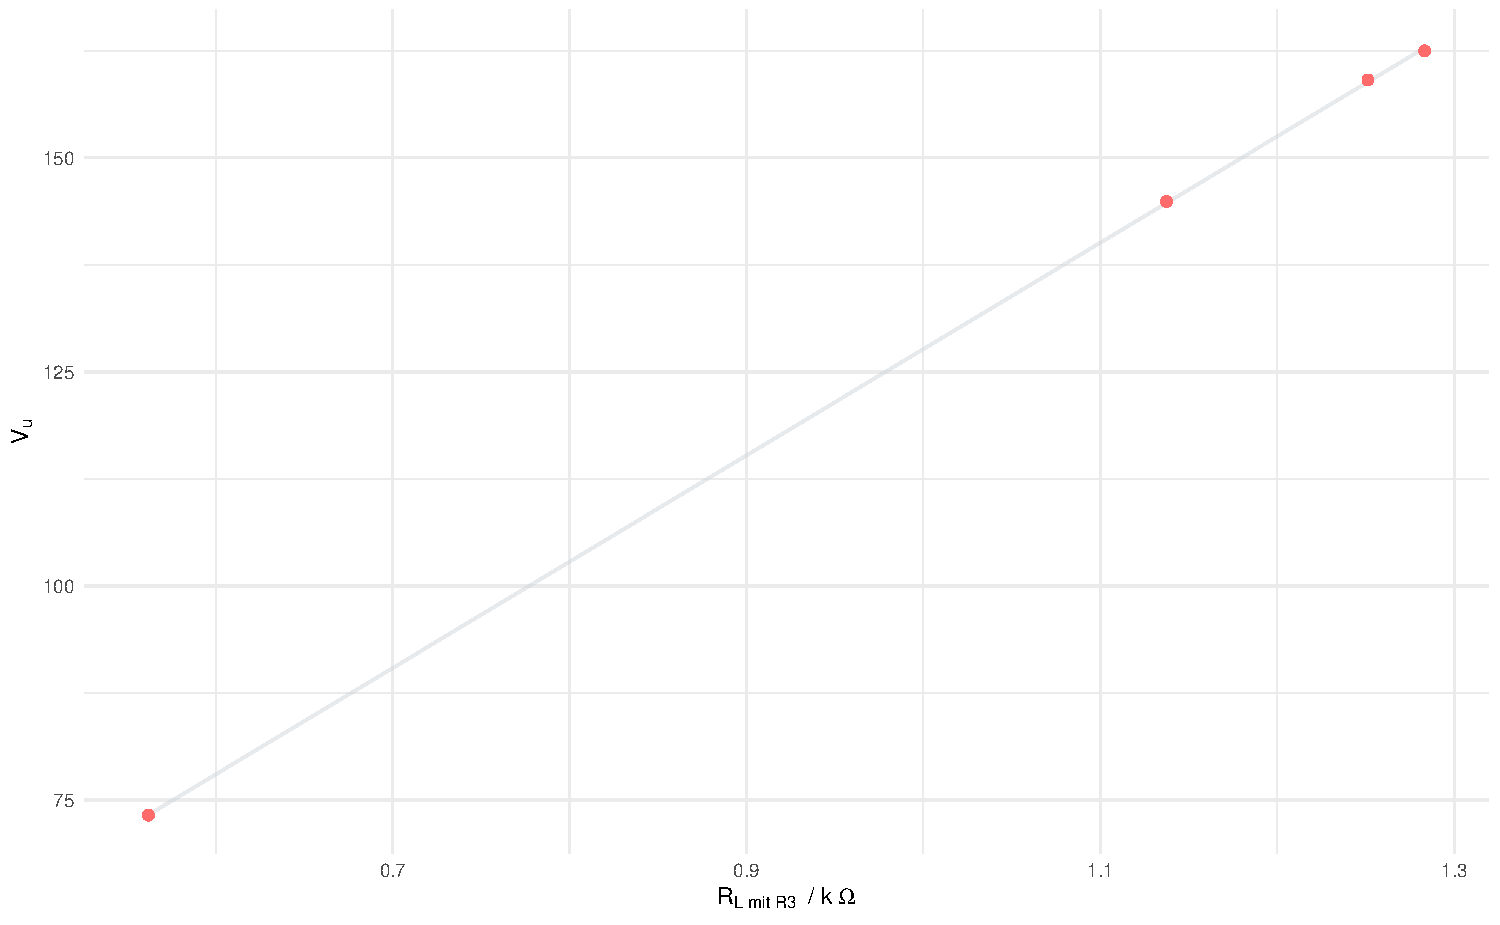
\includegraphics[width=\textwidth]{2_3/2_3_1_corrected.pdf}
  \end{center}
  \caption{Graph der Messwerte, korrigiert}
\end{figure}

Die resultierende Steilheit ist somit:
\[g_m \approx 128 \, \si{\milli\siemens}\]


(Da die Eingangsspannung den Kollektorstrom jedoch etwas verschiebt, ist die
Steilheit nicht konstant, was zu einer Abweichung des theoretisch linearen
Verhaltens führt. Außerdem wurde der Ausgangswiderstand des Transistors nicht berücksichtigt)

\subsubsection{Eingangswiderstand}
Mithilfe der U/2-Methode wurde der Eingangswiderstand der Schaltung bei
konstantem Lastwiderstand von $100 \, \si{\kilo\ohm}$ (kein externer Widerstand)
und einer Frequenz von $1 \, \si{\kilo\hertz}$ bestimmt.

\[U_{a1} = \frac{U_a}{2} = 413 \, \si{\milli\volt}\]

Der dabei ermittelte Eingangswiderstand ist
\[r_e = 800 \, \si{\ohm}\]

\begin{figure}[H]
  \begin{center}
    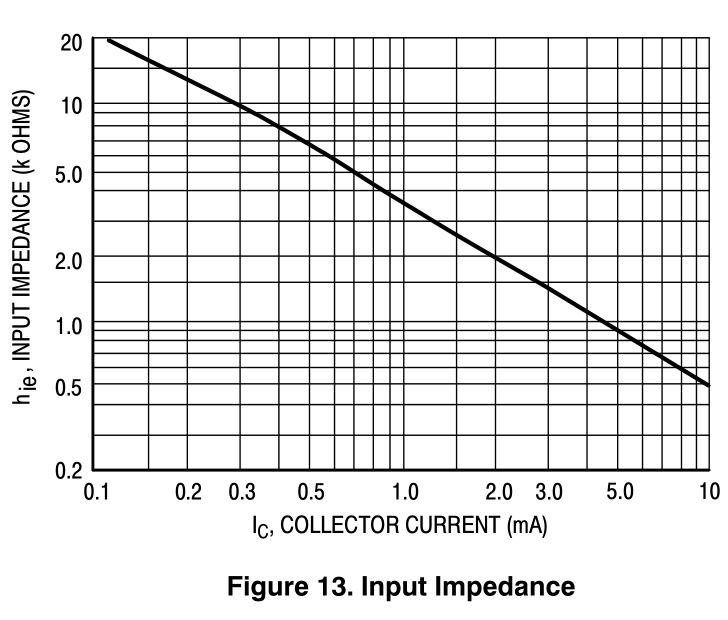
\includegraphics[width=0.618\textwidth]{inputimp}
  \end{center}
  \caption{Quelle: http://onsemi.com}
\end{figure}

Aus dem Transistordatenblatt Abb. 13 ist bei einem Kollektorstrom von $I_C = 4.33 \,
\si{\milli\ampere}$ ein $r_\pi$ von etwa $1 \, \si{\kilo\ohm}$ ablesbar. Der
theoretische Eingangswiderstand der Emitterschaltung ist
\[r_{e,\mathrm{theoretisch}} = R_1 // R_2 // r_\pi \approx 820 \,\si{\ohm}\]

Der messtechnisch ermittelte Wert stimmt also ziemlich genau mit dem
theoretischen überein. Mögliche Abweichungen entstehen durch ungenaue
Widerstandswerte, Messabweichungen/Fehlerfortpflanzung und ungenaues Ablesen von
Werten aus Datenblattkurven.

\subsubsection{Ausgangswiderstand}
Der Ausgangswiderstand bestimmt sich über die umgestellte Spannungsteilerformel
am Ausgangskreis. $U_{a0}$ ist die Leerlaufspannung, ohne Belastung. $U_{a1}$
die Ausgangsspannung bei Belastung mit dem externen Widerstand $R_L = 10 \, \si{\kilo\ohm}$.
\[U_{a1} = U_{a0} \cdot \frac{R_L}{r_a + R_L}\]
\[r_a = R_L \left( \frac{U_{a0}}{U_{a1}} -1 \right)\]

\[U_{a0} = 821.45 \, \si{\milli\volt}\]
\[U_{a1} = 731.50 \, \si{\milli\volt}\]

\[r_a = 10 \, \si{\kilo\ohm} \left( 821.45 \frac{ \, \si{\milli\volt}}{731.50 \,
      \si{\milli\volt}} -1 \right) = 1.2297 \, \si{\kilo\ohm}\]

\begin{figure}[H]
  \begin{center}
    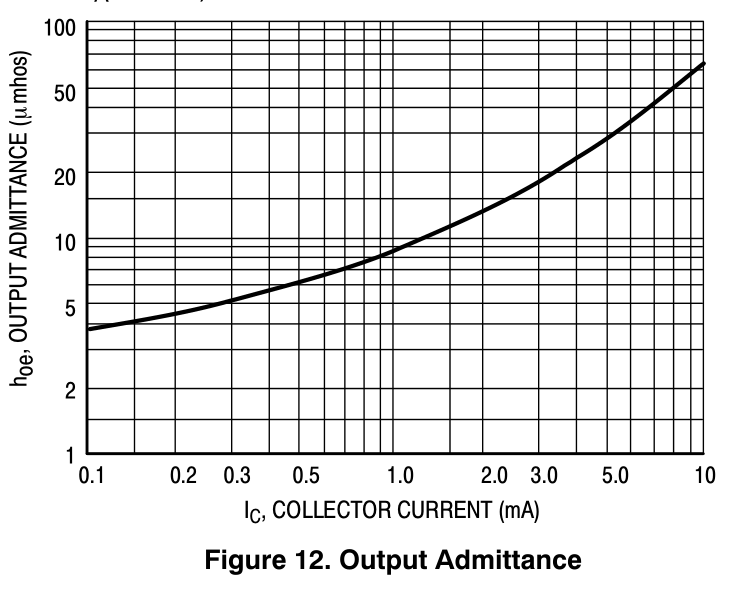
\includegraphics[width=0.618\textwidth]{outadmittance}
  \end{center}
  \caption{Quelle: http://onsemi.com}
\end{figure}

Der theoretische Ausgangswiderstandswert ergibt sich mit den Datenblattwerten zu
\[r_a = R_3 // R_L // r_0 = 1.3 \, \si{\kilo\ohm} // 100 \, \si{\kilo\ohm}// \, 33.33 \si{\kilo\ohm} \approx 1.236 \, \si{\kilo\ohm}\]

Der messtechnisch ermittelte Wert stimmt erneut gut mit dem theoretischen überein.

\subsubsection{Amplituden-Frequenzgang}
Der Amplituden-Frequenzgang wurde durch das Durchlaufen der
Eingangsspannungsfrequenzen von $0$ bis $10 \, \si{\kilo\hertz}$ und die Messung
der Ausgangsspannungswerte (RMS) bei einer Eingangsspannung von $U_e =
5\,\si{\milli\volt}_{\mathrm{RMS}}$ ermittelt.

\begin{figure}[H]
  \begin{center}
    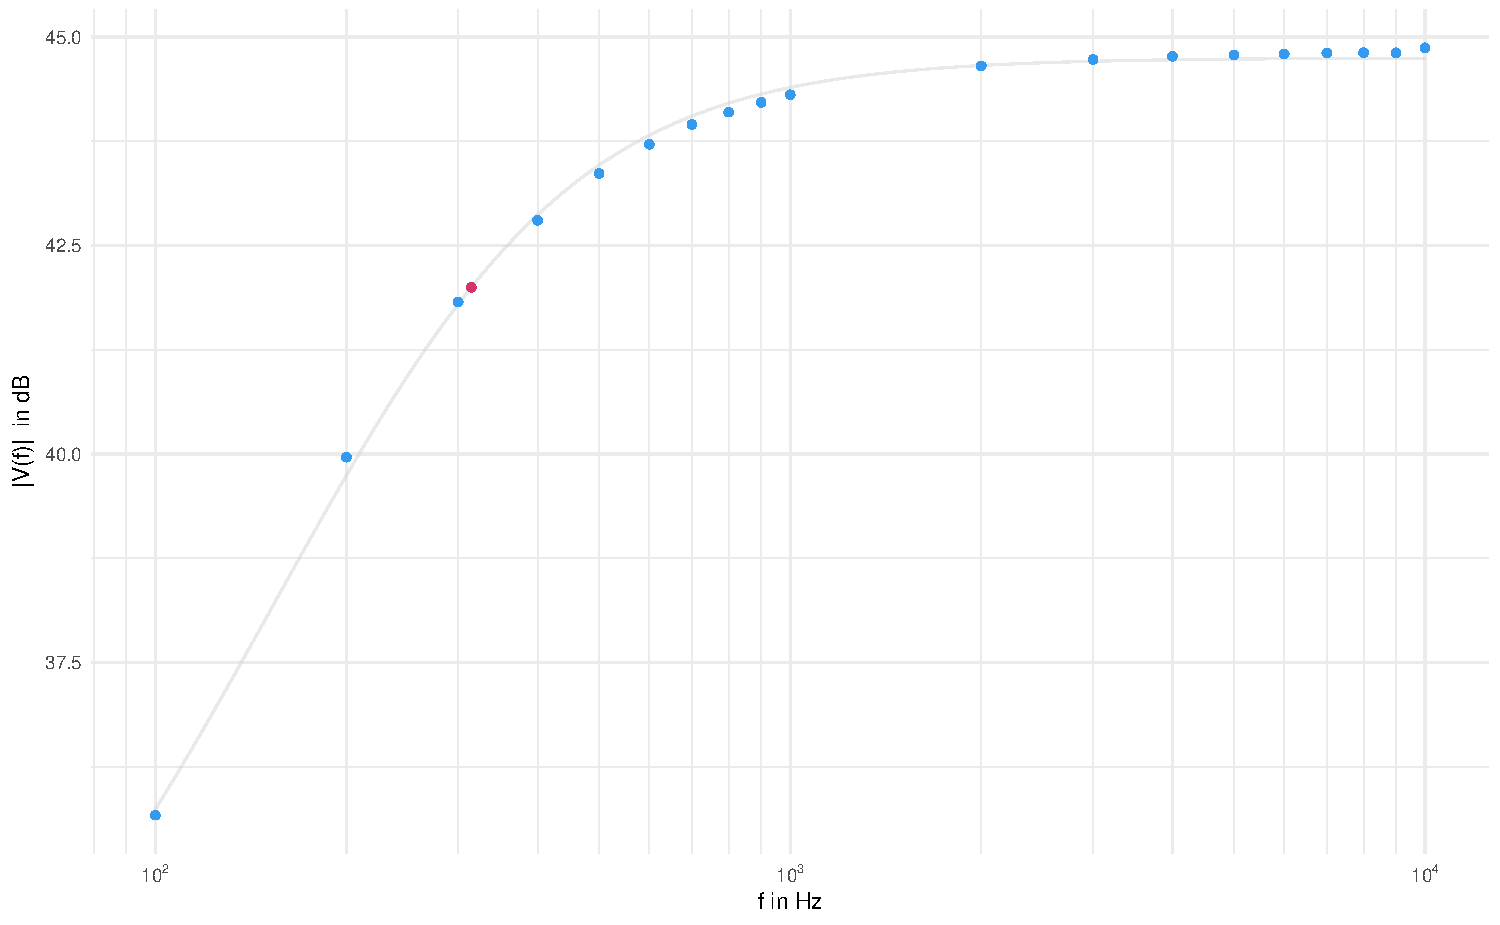
\includegraphics[width=\textwidth]{2_3/2_3_frequenzgang.pdf}
  \end{center}
  \caption{Amplitudenfrequenzgang der Messung}
\end{figure}

Die durch Regression ermittelte Grenzfrequenz ist
\[f_g \approx 300 \, \si{\hertz}\]

Vor der Grenzfrequenz steigt die Verstärkung mit etwa $25 \, \si{\deci\bel}$ pro
Dekade. Weit hinter der Grenzfrequenz nimmt sie den entsprechenden Wert aus
2.3.1 an.

$C_E$ ($C_3$) stellt wechselstromseitig einen Kurzschluss dar, wodurch der
Emitterwiderstand diesbezüglich wegfällt und die Verstärkung für 
Wechselspannungen deren Frequenz hoch genug ist nicht beeinflusst. Bei
niedrigeren Frequenzen ist die Reaktanz des Kondensators jedoch nicht
ausreichend gering, um den Einfluss von $R_E$ vollständig zu beseitigen, weshalb
die Verstärkung in diesem Fall sinkt.

\begin{table}[H]
\begin{center}
\begin{tabular}{@{}cc@{}}
\toprule
$f / \, \si{\hertz}$ & $u_\mathrm{a} / \, \si{\milli\volt}$ \\ \midrule
  \midrule
100                  & 303.7                       \\
200                  & 497.8                       \\
300                  & 616.8                       \\
400                  & 690.3                       \\
500                  & 736.5                       \\
600                  & 766.7                       \\
700                  & 787.9                       \\
800                  & 801.5                       \\
900                  & 812.38                      \\
1000                 & 820.96                      \\
2000                 & 854.3                       \\
3000                 & 862                         \\
4000                 & 865.7                       \\
5000                 & 867.5                       \\
6000                 & 868.6                       \\
7000                 & 869.6                       \\
8000                 & 870                         \\
9000                 & 870                         \\
10000                & 876                         \\ \bottomrule
\end{tabular}
\end{center}
\caption{Messwerte des Frequenzganges}
\end{table}

\subsection{Emitterschaltung mit Parallelgegenkopplung: ES\_IUGK1}
\subsubsection{Spannungsverstärkung}
Die Werte zur Bestimmung der Spannungsverstärkungen wurden bei einer
Eingangsspannung von $U_{\mathrm{RMS}} = 100 \, \si{\milli\volt}$ und einer
Frequenz von $f_e = 1 \, \si{\kilo\hertz}$ bestimmt. Der Lastwiderstand wurde
von $100 \, \si{\kilo\ohm}$ bis $1 \, \si{\kilo\ohm}$ variiert. Die
Spannungsverstärkungen bei den jeweiligen Lastwiderstandswerten ist dann
der Quotient aus Ausgangs- und Eingangsspannung. Die Spannungswerte wurden
als RMS-Werte am Oszilloskop gemessen. Der interne Lastwiderstand beträgt $R_{\mathrm{L,intern}} =
100 \, \si{\kilo\ohm}$.


\begin{table}[H]
  \begin{center}
    \begin{tabular}{|c|c|c|c|}
      \hline
      $U_e / \si{\milli\volt}$ & $U_a / \si{\milli\volt}$ & $R_{\mathrm{L,gesamt}} / \si{\kilo\ohm}$ & $V_u$\\
      \hline
      \hline
      99.92 & 1080 & 100 & 10.81\\
      99.95 & 1050 & 33.33 & 10.51\\
      99.93 & 954.5 & 9.09 & 9.55\\
      99.99 & 475.4 & 0.99 & 4.76\\
      \hline
    \end{tabular}
  \end{center}
  \caption{RMS-Spannungswerte und daraus resultierende Verstärkung bei
    verscheidenen Lastwiderständen (ohne $R_3$)}
\end{table}

\begin{figure}[H]
  \begin{center}
    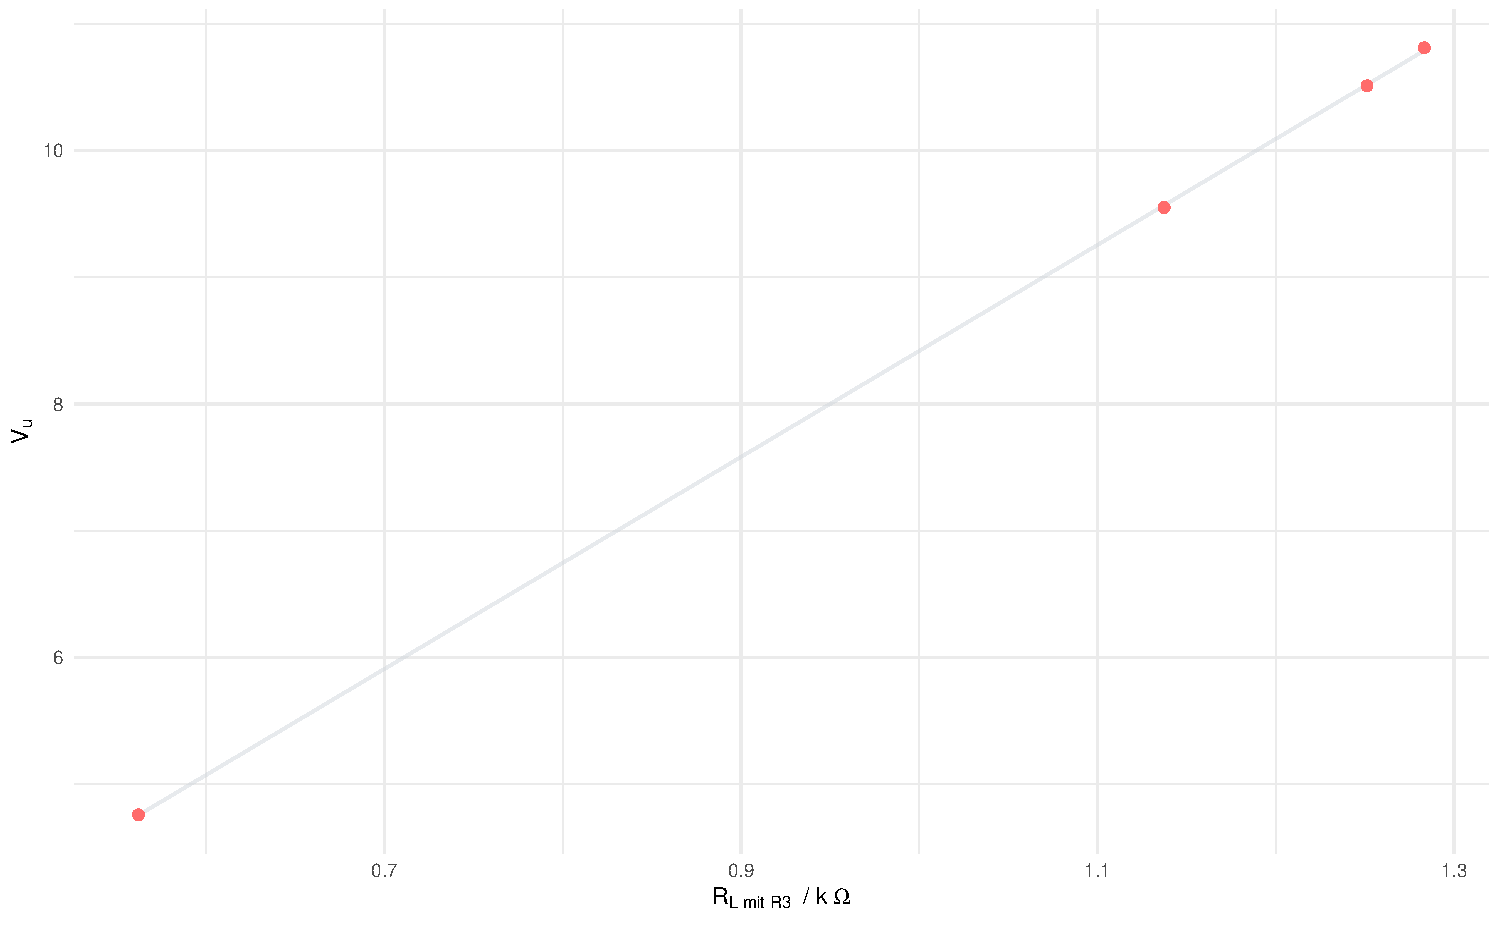
\includegraphics[width=\textwidth]{2_4/2_4_1_R3.pdf}
  \end{center}
  \caption{Graph der Messwerte, $R_3$ berücksichtigt}
\end{figure}

Der Zusammenhang zwischen Lastwiderstand und Verstärkung ist dem der vorherigen
Schaltung (ESIGK1) ähnlich. Die theoretische Steilheit des Transistors im Arbeitspunkt ist hier
\[g_{m,\mathrm{theoretisch}} = \frac{I_C}{U_T} = \frac{5.23 \, \si{\milli\ampere}}{26 \,
    \si{\milli\volt}} = 201.154 \, \si{\milli\siemens}\]

Durch die Gegenkopplung der Ausgangs- auf die Eingangsspannung wird, wie der
Versuch bestätigt, die Verstärkung der Emitterschaltung deutlich verringert.

\subsubsection{Eingangswiderstand}
Der Eingangswiderstand wurde auch hier nach der $U/2$-Methode bestimmt.

$U_{a0} = 1.08 \, \si{\volt}$
$U_{a1} = 500 \, \si{\milli\volt}$

Der dabei ermittelte Widerstandswert ist
\[r_e = 11 \, \si{\kilo\ohm}\]

Aus dem Datenblatt:
\[r_\pi = 0.9 \, \si{\kilo\ohm}\]
\[r_0 = 33.33 \, \si{\kilo\ohm}\]

Der theoretische Widerstandswert ist
\[r_{e} = R_2 // ((1+B_N) \cdot (R_5 // r_0) + r_\pi) = 21.35 \, \si{\kilo\ohm}\]

Der theoretische Wert ist etwa das Doppelte des theoretischen Wertes,
möglicherweise ist ein Rechen- oder Messfehler aufgetreten.

\subsubsection{Ausgangswiderstand}
Der Ausgangswiderstand wurde wie in 2.3.3 aus Messung zweier Spannungswerte
ermittelt. Der externe Ausgangslastwiderstand ist $R_L = 10 \, \si{\kilo\ohm}$

\[U_{a0} = 1080 \,\si{\milli\volt}\]
\[U_{a1} =  954.5 \,\si{\milli\volt}\]

\[r_a = 10 \, \si{\kilo\ohm} \left( \frac{1080 \, \si{\milli\volt}}{954.5 \,
      \si{\milli\volt}} -1 \right) \approx 1.3 \, \si{\kilo\ohm}\]





\subsection{Kollektorschaltung mit Bootstrap: KS\_BOS1}
\subsubsection{Spannungsverstärkungen}
Die Werte zur Bestimmung der Spannungsverstärkungen wurden bei einer
Eingangsspannung von $U_{\mathrm{RMS}} = 1 \, \si{\volt}$ und einer
Frequenz von $f_e = 1 \, \si{\kilo\hertz}$ bestimmt. Der Lastwiderstand wurde
von $100 \, \si{\kilo\ohm}$ bis $1 \, \si{\kilo\ohm}$ variiert. Der interne Lastwiderstand beträgt $R_{\mathrm{L,intern}} =
100 \, \si{\kilo\ohm}$.


\begin{table}[H]
  \begin{center}
    \begin{tabular}{|c|c|c|c|}
      \hline
      $U_e / \si{\milli\volt}$ & $U_a / \si{\milli\volt}$ & $R_{\mathrm{L,gesamt}} / \si{\kilo\ohm}$ & $V_u$\\
      \hline
      \hline
      997.7 & 995 & 100 & 0.9973\\
      1020 & 994 & 33.33 & 0.9745\\
      1020 & 992 & 9.09 & 0.9726\\
      1000 & 918 & 0.99 & 0.918\\
      \hline
    \end{tabular}
  \end{center}
  \caption{RMS-Spannungswerte und daraus resultierende Verstärkung bei
    verscheidenen Lastwiderständen}
\end{table}

Die Messung am Oszilloskop war sehr verrauscht, weshalb sich unter Umständen
starke Abweichungen ergeben können.

\begin{figure}[H]
  \begin{center}
    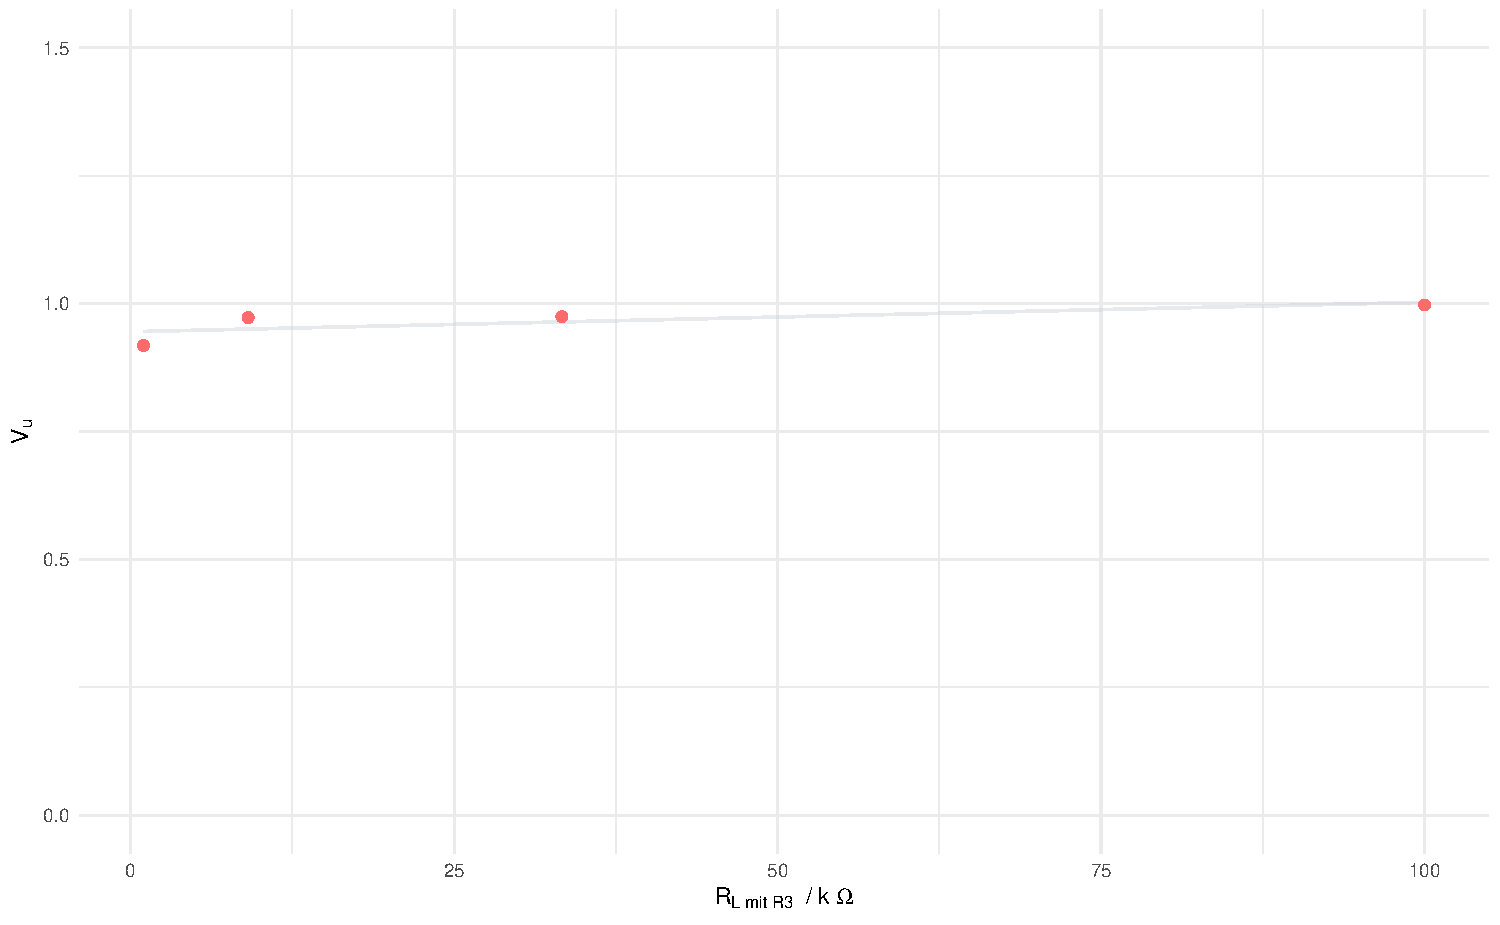
\includegraphics[width=\textwidth]{2_5/2_5_1.pdf}
  \end{center}
  \caption{Graph der Messwerte}
\end{figure}

Es lässt sich gut erkennen, dass die Verstärkereigenschaft der
Kollektorschaltung ($V_u \approx 1$) erfüllt ist.

\subsubsection{Eingangswiderstand}
Der theoretische Wert des Eingangswiderstandes der Kollektorschaltung ohne
Bootstrap, d.h. wenn $R_3 = 0$ und C weggelassen wird,  ist ( mit $B = 294$ im Arbeitspunkt)
\[r_{e,\mathrm{noBT}} = R_1 // R_2 // (B \cdot (R_4 // R_5)) = 184.5 \,\si{\kilo\ohm}\]

Messtechnisch konnte der Eingangsreihenwiderstand für die U/2 Methode nicht auf
einen ausreichend hohen Wert gestellt werden, da die verwendetete
Widerstandsdekade dies nicht hergab.

\subsubsection{Ausgangswiderstand}
Wie in den vorherigen Aufgaben ist der Ausgangswiderstand (bei einem
Lastwiderstand von $10 \, \si{\kilo\ohm}$)

\[r_a = R_L \left( \frac{U_{a0}}{U_{a1}} -1 \right)\]
\[r_a = 10 \, \si{\kilo\ohm} \left( \frac{995 \, \si{\milli\volt}}{993 \,
      \si{\milli\volt}} -1 \right)= 30.24 \, \si{\milli\ohm}\]

Der Ausgangswiderstand der Kollektorschaltung ohne Bootstrap, mit den gleichen
restlichen Widerstandswerten, ($I_C = 1.299 \, \si{\milli\ampere}$ (LTSPICE)) ist
\[r_a \approx \frac{1}{g_m} = \frac{U_T}{I_C} = \frac{26 \,
    \si{\milli\volt}}{1.299 \, \si{\milli\ampere}} = 20.02 \, \si{\ohm}\]

\subsection{Vergleich der Grundschaltungen}
\begin{table}[H]
\centering
\caption{Qualitativer Vergleich der Grundschaltungen mit Beispielwerten}
\label{my-label}
\begin{tabular}{|*{4}{p{0.25\textwidth}|}}
\hline
Schaltung     & Emitterschaltung & Kollektorschaltung & Basisschaltung \\ \hline
  \hline
Spannungsverstärkung   &    hoch      & $\approx< 1$            & hoch (wie Emitterschaltung) \\ \hline
Eingangswiderstand &   durchschnittlich ($\approx 1 \, \si{\kilo\ohm}$)       &  am höchsten ($\approx 100 \, \si{\kilo\ohm}$)           &      gering $\approx 50 \, \si{\ohm}$      \\ \hline
Ausgangswiderstand  &  durchschnittlich $\approx 50 \, \si{\kilo\ohm}$        &            gering $\approx 200 \,\si{\ohm}$&  sehr hoch $\approx 1 \, \si{\mega\ohm} $       \\ \hline
Bsp. Einsatzgebiet        &      allg. Verstärkerschaltung    &   Impedanzwandler         &    Hochfrequenzverstärker (hohe Grenzfrequenz)        \\ \hline
\end{tabular}
\end{table}

\end{document}
